%% 
%% Copyright 2019-2021 Elsevier Ltd
%% 
%% This file is part of the 'CAS Bundle'.
%% --------------------------------------
%% 
%% It may be distributed under the conditions of the LaTeX Project Public
%% License, either version 1.2 of this license or (at your option) any
%% later version.  The latest version of this license is in
%%    http://www.latex-project.org/lppl.txt
%% and version 1.2 or later is part of all distributions of LaTeX
%% version 1999/12/01 or later.
%% 
%% The list of all files belonging to the 'CAS Bundle' is
%% given in the file `manifest.txt'.
%% 
%% Template article for cas-sc documentclass for 
%% single column output.

% Document Class
\documentclass[a4paper,fleqn]{cas-sc}

% Packages
%%\usepackage[authoryear,longnamesfirst]{natbib}
\usepackage[numbers]{natbib}
\usepackage[nodots,nocompress]{numcompress}

%Package to hold figure in position
\usepackage{placeins}

%Author macros
\def\tsc#1{\csdef{#1}{\textsc{\lowercase{#1}}\xspace}}
\tsc{WGM}
\tsc{QE}

\begin{document}
\let\WriteBookmarks\relax
\def\floatpagepagefraction{1}
\def\textpagefraction{.001}

% Short title
\shorttitle{Numerical analysis of the rock deformation in twin tunnels with transverse gallery}    

% Short author
\shortauthors{Quevedo et al.}  

% Main title of the paper
\title [mode = title]{Numerical analysis of the rock deformation in twin tunnels with transverse gallery considering plasticity and time-dependent constitutive models}  

% First author
\author[1]{Quevedo, F. P. M.}[style = chinese, orcid = 0000-0003-4171-1696]
\cormark[1] 					
\cortext[cor1]{Corresponding author.}
\ead{motta.quevedo@ufrgs.br}
\ead[url]{https://www.researchgate.net/profile/Felipe-Pinto-Da-Motta-Quevedo}

% Second author
\author[1]{Colombo, C. A. M. M.}[style=chinese]
\ead{ca-colombo@hotmail.com}
\ead[url]{http://lattes.cnpq.br/4919388217690564}

% Third author
\author[1]{Bernaud, D.}[style=chinese, orcid=0000-0001-6365-3269]
\ead{denise.bernaud@ufrgs.br}
\ead[url]{http://lattes.cnpq.br/2809615143819128}

% Four author
\author[1]{Maghous, S.}[style=chinese, orcid=0000-0002-1123-3411]
\ead{samir.maghous@ufrgs.br}
\ead[url]{https://www.researchgate.net/profile/Samir-Maghous}

% Afilliation
\affiliation[1]{organization={Federal University of Rio Grande do Sul},
	addressline={Av. Osvaldo Aranha, 99}, 
	city={Porto Alegre},
	postcode={90.035-190}, 
	state={RS},
	country={Brazil}}

% Mathematical Symbols
\newcommand{\dgds}{\boldsymbol{g_\sigma}}
\newcommand{\Dll}{\boldsymbol{D}}
\newcommand{\Dllmod}{\boldsymbol{D^{*}}}
\newcommand{\Dllepvp}{\boldsymbol{D}^{epvp}}
\newcommand{\dstrain}{\boldsymbol{\dot{\varepsilon}}}
\newcommand{\dstraine}{\boldsymbol{\dot{\varepsilon}}^{e}}
\newcommand{\dstrainp}{\boldsymbol{\dot{\varepsilon}}^{p}}
\newcommand{\dstrainv}{\boldsymbol{\dot{\varepsilon}}^{vp}}
\newcommand{\straineqp}{\bar \varepsilon^p}
\newcommand{\dstrainsh}{\boldsymbol{\dot{\varepsilon}}^{sh}}
\newcommand{\dstraincr}{\boldsymbol{\dot{\varepsilon}}^{cr}}
\newcommand{\dstress}{\boldsymbol{\dot{\sigma}}}

\newcommand{\ex}{\boldsymbol{e}_x}
\newcommand{\ey}{\boldsymbol{e}_y}
\newcommand{\ez}{\boldsymbol{e}_z}

\newcommand{\onell}{\boldsymbol{1}}
\newcommand{\strain}{\boldsymbol{\varepsilon}}
\newcommand{\straincr}{\boldsymbol{\varepsilon}^{cr}}
\newcommand{\straine}{\boldsymbol{\varepsilon}^{e}}
\newcommand{\strainp}{\boldsymbol{\varepsilon}^{p}}
\newcommand{\strainsh}{\boldsymbol{\varepsilon}^{sh}}
\newcommand{\strainshCEB}{\varepsilon_{sh}}
\newcommand{\strainvp}{\boldsymbol{\varepsilon}^{vp}}
\newcommand{\stress}{\boldsymbol{\sigma}}
\newcommand{\zerol}{\boldsymbol 0}

% Here goes the abstract
\begin{abstract}
Resorting a three-dimensional finite element analysis, this paper investigates the instantaneous and long-term implications induced by the time-dependent constitutive behavior of constituents on the convergence profile of twin tunnels linked with transverse galleries. Several constitutive models for rock mass mechanical behavior are examined at the material level, encompassing elastoplasticity, viscoplasticity, or coupled elastoplasticity-viscoplasticity frameworks. Plasticity state equations are based on a Drucker-Prager yield surface with an associated flow rule, while the viscoplasticity formulation relies on the Perzyna model with a Drucker-Prager flow surface. Tunnel lining behavior is modeled using either elastic or viscoelastic constitutive models. The viscoelastic behavior is described by a Generalized Kelvin rheological model based on Bazant and Prassanann's Solidification Theory, with model parameters derived from CEB-FIP MC90 formulations. From a computational viewpoint, the deactivation-activation method is employed to simulate the excavation process and lining installation. The accuracy of finite element predictions is assessed through comparisons with available analytical solutions formulated in a simplified setting for the twin tunnels' configuration. A parametric study delves into the mutual interaction induced by tunnels proximity, emphasizing the crucial role of concrete lining stiffness in twin tunnels' deformation. Numerical simulations indicate a highly localized influence of a transverse gallery on twin tunnels deformation, extending up to four radii from each side of the gallery axis. Finally, the paper investigates the effects of twin tunnels proximity and those induced by an interconnecting gallery on the instantaneous and long-term convergence of tunnels, contrasting these outcomes with the convergence of a single tunnel.
\end{abstract}

% Use if graphical abstract is present
\begin{graphicalabstract}
	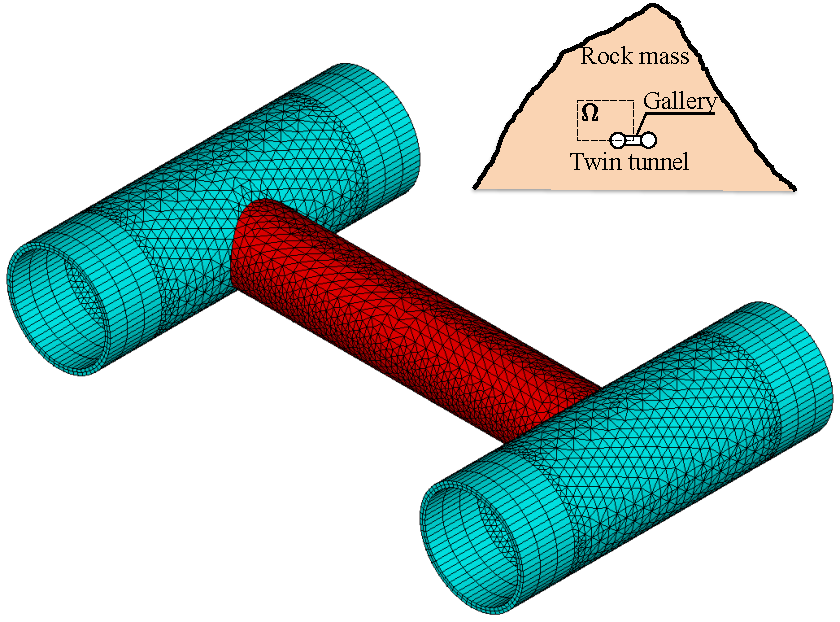
\includegraphics[scale=1]{graphical_abstract.pdf}
\end{graphicalabstract}

% Research highlights
\begin{highlights}
	\item The stiffness of the lining restricting viscous effects in the interaction of tunnels
	\item Interaction between the tunnels becomes significant at a span distance of 4 radii
	\item The viscous of the concrete lining can be important in the tunnel convergence
	\item The effect of the gallery extends into the tunnel up to 4 radii from its axis
	\item The proximity of the tunnels induces the ovalization of the tunnel wall 
\end{highlights}

% Keywords
\begin{keywords}
twin tunnels \sep transverse gallery \sep elastoplasticity-viscoplasticity coupling
\sep viscoelastic lining \sep finite element method
\end{keywords}

\maketitle

\section{Introduction}\label{}

Many design methods often focus on single tunnels, but twin tunnels are a common occurrence. The interaction between tunnels can be significant, especially when the spacing between them is minimal. Additionally, many twin tunnels incorporate transverse galleries, introducing a localized effect on displacements and stresses. Also, the rheological behavior of the rock mass and lining plays a crucial role in how stress and displacements fields evolve over time. Some recent studies on deep twin tunnels can be found at [\citenum{Spyridis2015}, \citenum{Chen2019}, \citenum{Fortsakis2021}, \citenum{chortis2021a}, \citenum{chortis2021b}, \citenum{GUO2021}, \citenum{chortis2023a}, \citenum{chortis2023b}].

Chortis and Kavvadas [\citenum{chortis2021a}] considered the calculation of the axial forces acting on the primary support in the intersection zone before, during, and after the construction of a perpendicular tunnel intersection. The results of the analysis indicated that the zone of influence extends approximately two diameters from the main tunnel to each side from the center of the intersection and that the interaction effects are practically eliminated when they exceed this influence zone. 

In another study, Chortis and Kavvadas [\citenum{chortis2021b}] carried out parametric 3D finite element analyses to verify the interaction between deep twin tunnel, with circular and non-circular cross-section, supported by a shotcrete elastic linear lining. Was considering the rock mass with linear elastic behavior and perfectly plastic, with Mohr-Coulumb failure criteria. The study investigates the axial forces that develop in the primary lining of the twin tunnels as a function of the main geometric and geomaterial parameters, but without considering the potential time-dependent deformations (creep effect) that occur in some types of rock masses.

Chen et al. [\citenum{Chen2019}], through analytical solutions in elasticity using complex variables, Fourier transformation, and the alternating Schwarz method, demonstrate that the mutual interaction between twin tunnels disappears if the spacing between the tunnels is greater than six times the tunnel radius. The lining effectively reduces the stress concentration, especially at high lateral stress coefficients.

Guo et al. [\citenum{GUO2021}] develop an elastic analytical solution for the stress field around twin circular tunnels with hydrostatic pressure using the complex variable and the superposition principle. They found that stress concentration in tunnel wall increased as the distance between the parallel tunnels decreased and the supporting pressure leads to the radial stress increasing and the tangential stress decreasing.

Ma et al. [\citenum{MA2020}] proposed an analytical method, verified by a numerical solution using FLAC3D software for determining the plastic zones around deep circular twin tunnels without linings, restricting themselves where there is no overlap between the two plastic zones. In this case, the authors adopted the elastoplastic perfectly constitutive model for the homogeneous and isotropic rock mass, with the Mohr-Coulomb criterion. Also carried out parametric studies to understand the influence of the distance between the twin tunnels, cohesion, the angle of internal friction, and the vertical and horizontal initial stresses acting on the shape and depth of the plastic zones. These authors stated that the plastic zone around the tunnel provides a relevant theoretical basis for defining and designing the support. In that respect, an excessive plastic zone would significantly affect the stability and functionality of a tunnel. Reducing the extension of the plastic zone around tunnels is, therefore, of great importance in engineering tunnel design projects.

Using parametric three-dimensional numerical analyses, Chortis and Kavvadas [\citenum{chortis2023a}, \citenum{chortis2023b}] investigated the effect of building a transverse tunnel that intersected deep twin tunnels perpendicularly, focusing the study on the axial forces and the circumferential and longitudinal bending moments acting on the primary support of the intersection regions, respectively. According to the authors, the potential interaction between deep twin tunnels lined with shotcrete must be taken into account, especially when the distance between them is less than or equal to twice their diameter.

According to Fortsakis [\citenum{Fortsakis2021}], in a realistic construction context, twin tunnels are excavated and supported with a delay, so that the second tunnel is usually built after the first one has advanced enough to maintain a longitudinal separation distance between the faces. The advance of the subsequent tunnel mobilizes the redistribution of stresses and deformations in the zone between the tunnels, resulting in additional loading of the preceding tunnel.

As for transverse tunnels, these are generally built far enough behind the advanced face of the main tunnel to ensure that their excavation has virtually no effect during the construction of the junction tunnel [\citenum{chortis2021a}]. The interaction at the intersection, between the main tunnel and the transverse tunnel, significantly modifies the stress state of the primary support and that of the surrounding rock mass in these areas, compared to that of the singular tunnel, making three-dimensional finite element analyses essential for developing a realistic and safe design for tunnel junctions [\citenum{Spyridis2015}].

During the construction of the transverse tunnel, the surrounding rock mass is subjected to a redistribution of stresses, causing an additional load on the main tunnel, precisely in the intersection zone. If these additional loads exceed the load capacity of the primary support of the main tunnel, a potentially unstable region can develop, leading to failure, especially in adverse geotechnical conditions [\citenum{chortis2021a}].

While the simulation of tunnel convergence in single tunnels has been widely investigated and reported in published literature, few works have addressed the computational evaluation of deformation in twin tunnels. Less attention has been dedicated to assessing the mutual mechanical interaction induced by the excavation of the transverse gallery connecting the twin tunnels. 

In this context, the main contributions of this paper may be summarized at both the material and tunnel analysis levels. At the material level, the constitutive state equations of the rock mass are formulated within the framework of coupled plasticity-viscoplasticity, which is relevant for clayey rocks. Such a framework allows capturing the irreversible instantaneous tunnel response (plasticity) as well as the delayed irreversible response (viscoplasticity).  As regards the mechanical behavior of concrete material defining the lining, which is classically modeled through linear elastic relationships, the present analysis considers an aging viscoelastic rheological model relying upon the Bažant and Prasannan Solidification theory [\citenum{bazant:1989a,bazant:1989b}]. At the structure analysis level, the simulation of deformation in the highly interacting material system components (namely, rock mass and lining), resulting from the excavation process of twin tunnels and transverse gallery, is handled using finite element simulations performed in a three-dimensional setting. From the computational viewpoint, the excavation process and lining placement are simulated by means of the activation/deactivation technique. The constitutive models formulated for the rock mass and lining constituent as well as the related numerical integration schemes are implemented into the same procedure UPF/USERMAT customization tool [\citenum{ANSYS:2013b}] of ANSYS standard software. The three-dimensional finite element analysis developed in this paper is specifically devised for addressing the three-dimensional interaction induced by the construction process, twin tunnels proximity, and the presence of the transverse gallery.

\section{Fundamental assumptions}\label{}

The basic assumptions of the constitutive and computational modeling, as well as related limitations, are summarized as follows:

\begin{enumerate}[(a)]
	\item Only the configuration of deep tunnels shall be considered in the subsequent analysis, thus neglecting deformations caused by surface loads and settlements arising from the excavation process.

	\item Although material heterogeneity and behavior anisotropy are inherent features of soils and rocks, the rock mass is modeled throughout the paper as a homogeneous and isotropic continuous medium. At the scale adopted for tunnel modeling (macroscopic scale), this assumption means in particular that the possible micro-heterogeneities, such isotropic distributions of joints or cracks present at the finer scale, are accounted for in the homogenized behavior by means of a preliminary homogenization process (e.g., [\citenum{nemat1993}, \citenum{deude2002}, \citenum{deBuhan2002}, \citenum{Marmier2007}, \citenum{Aguiar2023}]). Clearly enough, the framework of continuum modeling adopted in the paper would reveal questionable when the rock mass is cut by a few macroscale fracture joints.  
	
	\item The rock mass is phenomenologically modeled using an elastoplastic-viscoplastic rheological law to capture instantaneous and long-term responses. This approach disregards the aspect connected temperature gradients, water flow, and poromechanics coupling.

	\item Despite the complexity of the stress distribution prevailing in the rock mass before the process of tunnel excavation, which is mainly affected by the geological history, the present study assumes a geostatic initial stress reflected by vertical and horizontal stresses.

	\item Twin tunnels are often designed considering a time gap between excavation fronts. However, the finite element simulations assume synchronous excavation steps to ensure symmetry conditions.

	\item The simulation excavation processes are curried out assuming a constant tunnel advancement rate (i.e., constant excavation speed), together with a constant thickness of concrete lining.
	
	\item Effects of temperature and humidity that may affect the viscoelastic behavior of lining concrete are disregarded.
	
	\item Perfect bonding is assumed at the interface between concrete lining and the rock mass.

	\item The framework of infinitesimal strain analysis, together with quasi-static evolutions, is adopted in the paper. In particular, dynamic excitations and related inertial forces, such as those induced, for instance, by earthquakes or explosions, shall not be considered in the numerical analysis.
	
\end{enumerate}

\section{Constitutive Model of the Rock Material}\label{}

Time-dependent phenomena associated with the delayed behavior of the constitutive material are key aspects of deformation in tunnel structures excavated in deep clayey rocks (see for instance [\citenum{rousset1988}, \citenum{Nguyen1987}] or [\citenum{GIRAUD1996}], to cite a few). In most computational analyses developed for tunnel engineering design, this issue is generally addressed by means of viscoplastic constitutive behavior. While such constitutive models could relevantly model the transient and long-term deformation, they seem however inadequate to capture the influence of short-term events (tunnelling and support placement phases) on the final stability of the structure. In particular, an analysis of tunnel deformation based on a viscoplastic model would suggest that the ultimate support pressure at tunnel structure equilibrium mainly depends on the closure rate at the moment when the contact between lining and rock mass is achieved (e. g., [\citenum{Nguyen1987}]), thus disregarding the irreversible effects rising in the initial construction phases. Indeed, during the primary stages of tunnel excavation, the surrounding rock mass is subjected to severe loading conditions and high strain rates, which may lead to yielding associated with high instantaneous irreversible strains near the tunnel wall, and can therefore affect the long-term equilibrium of the structure. It is thus of fundamental concern to formulate a constitutive model that incorporates both instantaneous and delayed irreversible components of the rock material. For this purpose, the present analysis considers a constitutive model that includes both instantaneous plasticity to describe shorth-term material yielding and viscoplasticity to represent delayed behavior. The formulation of the coupled plasticity-viscoplasticity rheological model is based on that originally proposed in [\citenum{Nguyen1987}] and [\citenum{rousset1988}]. Previous studies have implemented this plastic-viscoplastic model for computational analysis of deformation in single tunnels (e.g., [\citenum{Bernaud1993}, \citenum{piepi1995}, \citenum{GIRAUD1996}, \citenum{quevedo2022thesis}]. For the sake of brevity, only the main features of this constitutive model shall be summarized below.  Detailed description of the model, including application and validation in the context of single tunnel structures may be found in [\citenum{quevedo2022b}]. Finite element implementation of this model in the USERMAT procedure of  ANSYS software is also described in [\citenum{quevedo2022thesis}].

The elastoplastic-viscoplastic model is formulated based on a serial association of the elastoplastic and viscoplastic constitutive models. The local strain rate $\dstrain$ is split into three contributions $\dstrain = \dstraine + \dstrainp + \dstrainv$, so that the constitutive relationships relating the Cauchy stress rate $\dstress$ and strain rate components can be written as:
\begin{equation} \label{eq_constitutive_relationship_epvp}
	\dstress = \Dll : \dstraine = \Dll : (\dstrain - \dstrainp - \dstrainv).\;
\end{equation}

In the above relationship, $\dstraine$, $\dstrainp$ and $\dstrainv$, represent respectively the elastic, plastic and viscoplastic strain rate, and $\Dll$ denote the fourth-order isotropic elastic linear constitutive tensor. Tensor $\Dll$ is defined by the rock mass elastic Young modulus $E$ and Poisson ratio $\nu$. The one-dimensional representation of the constitutive behavior is shown in Fig.~\ref{reological_scheme}.
\begin{figure}[h!]
	\centering
	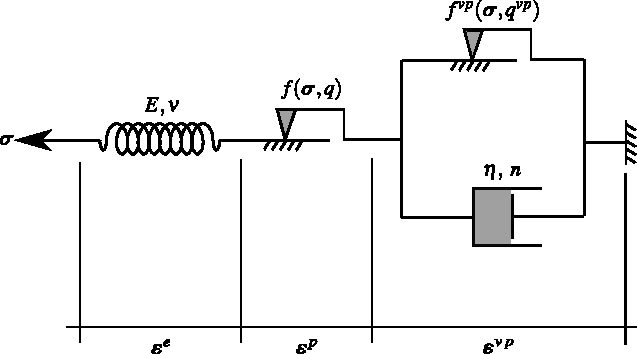
\includegraphics[scale=1]{Rheological representation.pdf}
	\caption{Rheological representation of the elastoplastic-viscoplastic model.}
	\label{reological_scheme}
\end{figure}
\FloatBarrier
In the three-dimensional context, the plasticity component of constitutive behavior is described by a Drucker-Prager plastic flow surface given by:
\begin{equation}
	\label{eq:f_Drucker_Prager}
	f(\stress,q) = f(I_1,J_2,q) = \beta_1 I_1 +\beta_2 \sqrt{J_2}-q(\alpha),
\end{equation}
which $I_1$ is the first invariant of the stress tensor, $J_2$ the second invariant of the deviator tensor and $\beta_1, \beta_2$ and $q(\alpha)$ are strength parameters related to the friction angle $\phi$ and cohesion $c(\alpha)$, respectively. Drucker-Prager plasticity surface inscribed to the Mohr-Coulomb surface shall be considered throughout the subsequent analysis [\citenum{bernaud1991}]:
\begin{equation}
	\label{eq:f_DP_inscrita_MC}
	\beta_1 = \dfrac{(k-1)}{3}, ~~~ \beta_2 = \dfrac{(2k+1)}{\sqrt{3}}, ~~~
	q(\alpha) = 2\sqrt{k}~c(\alpha),
\end{equation}
where $k = (1+\sin{\phi})/(1-\sin{\phi})$. The internal variable $\alpha$ is the equivalent plastic strain $\straineqp$ used to simulate strain hardening/softening phenomena. However, for this study, we adopt perfect plasticity, meaning that c is a constant. For the viscoplasticity surface $f^{vp}$ the same surface is empolyed, but with $\phi^{vp}$ in $\beta_1$ and $\beta_2$, and $q^{vp} = 2\sqrt{k^{vp}}-c^{vp}$ where $k^{vp} = (1+\sin{\phi^{vp}})/(1-\sin{\phi^{vp}})$ and $c^{vp}$ is a constant, i.e., perfect viscoplasticity. 
The plastic flow rule is given by:
\begin{equation}
	\label{eq_plastic_flow}
	\dot \strainp = \left\{ 
	\begin{array}{ll} 
		\dot \lambda \dfrac{\partial g}{\partial \stress} &  \text{for } f > 0 \\ 
		\zerol, & \text{for } f \le 0 \\
	\end{array}\right.,
\end{equation}
where $\dot \lambda$ is the plasticity multiplier and $g$ is a potential flow function analogous to $f$ used to simulate the volume dilatation during the evolution of plastic deformations. However, for this analysis, was used associated plasticity, i.e., $g=f$. The plastic multiplier is obtained through the consistency condition $\dot f = 0$. Numerical details of this implementation can be found in [\citenum{quevedo2022b}]. For viscoplastic flow rule we have,
\begin{equation}
	\label{eq_viscoplastic_flow}
	\dstrainv = \dot \lambda^{vp} \dfrac{\partial f^{vp}}{\partial \stress}
\end{equation}
In contrast to the plastic multiplier, the viscoplastic multiplier $\lambda^{vp}$ is independent of a consistency like condition. As a result, its expression is explicit. Based on the framework of generalized Perzyna's overstress theory [\citenum{perzyna1966}], its expression may be derived as follows:
\begin{equation} \label{eq_perzyna_model}
	\dot \lambda^{vp} = \dfrac{\Phi(\stress,q^{vp})}{\eta}~~~\text{and}~~~\Phi = \left\langle  \dfrac{f^{vp}(\stress,q^{vp})}{f_0} \right\rangle^n, \,
\end{equation} where $\Phi$ is the overstress function, $\eta$ is the dynamic viscosity constant, $n$ is the dimensionless parameter that gives the form of the power law, $f_0$ a parameter conveniently adopted and $\left\langle * \right\rangle$ is the McCauley function which is $0$ when $* <0$ , i.e. viscoplastic flow will only occur when the overstress function is positive.

In this coupled model, when $\phi=\phi^{vp}$, cohesion entirely controls the evolution of local mechanical fields. Specifically, when  $c \rightarrow \infty$ and $c^{vp} \rightarrow \infty$, the system achieves a purely elastic solution. The solution becomes purely elastoviscoplastic with $c \rightarrow \infty$, while a pure elastoplastic solution emerges with $c^{vp} \rightarrow \infty$. In the coupled analysis, condition $c^{vp} < c$ is adopted, allowing the viscoplastic domain to occur without plasticity. However, in the presence of plasticity, viscous effects become inevitable. Fig.~\ref{epvpdomains} illustrates these domains in principal stress space.
\begin{figure}[h!]
	\centering
	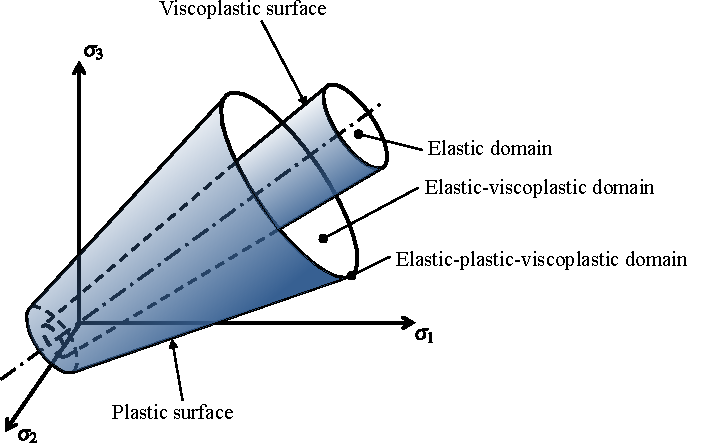
\includegraphics[scale=0.8]{Elastic-plastic-viscoplastic domains.pdf}
	\caption{Elastoplastic-viscoplastic domains.}
	\label{epvpdomains}
\end{figure}

\section{Constitutive Model of the Lining}\label{}

Shrinkage and creep phenomena represent fundamental components of concrete deformation processes that are expected to naturally affect the instantaneous as well as the transient and long-term behavior of structures involving such material. However, most of the tunnel design analyses consider the concrete involved in lining systems as a linear elastic material. From a phenomenological point of view, creep of concrete refers to the time-dependent deformation induced by sustained loading, whereas shrinkage deformation refers to the volume decrease caused by drying. As far as deformation in tunnel structures is concerned, creep and shrinkage have an important effect on the performance of the concrete lining and consequently on its contribution to controlling the long-term convergence of the tunnel. To account for such constitutive features, the concrete creep deformation is addressed by means of an aging viscoelastic rheological model relying on Bažant and Prasannan Solidification Theory [\citenum{bazant:1989a},  \citenum{bazant:1989b}]. The viscoelastic model is described by a Generalized Kelvin-chain as depicted in Fig.~\ref{reological_representation_concrete}. The mechanical parameters that define such a rheological model are the springs stifness and dash-pots viscosity. The model parameters are calibrated based on the CEB-FIP MC90 standard specifications formulation reported in [\citenum{CEB:1993}]. One may refer to [\citenum{quevedo2018} , \citenum{quevedo2022}] for detailed description of the calibration procedure. As regards the concrete deformation associated with shrinkage, the isotropic formulation proposed in CEB-FIP MC90 standard [\citenum{CEB:1993}] is adopted in the present modeling and subsequent computational analyses. Full details regarding model definition and related finite element implementation may be found in [\citenum{quevedo2017comportamento}] and [\citenum{quevedo2022}].

\begin{figure}[h!]
	\centering
	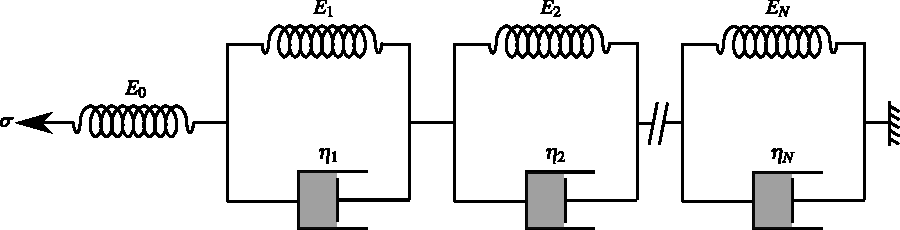
\includegraphics[scale=1]{Rheological_representation_concrete.pdf}
	\caption{Generalized Kelvin model for uniaxial concrete viscoelasticity.}
	\label{reological_representation_concrete}
\end{figure}

Accordingly, the constitutive equations for concrete lining relating the stress and strain rate can be expressed in the framework of infinitesimal strain analysis as:
\begin{equation} \label{eq:8}
	\dstress = \Dll : \dstraine = \Dll : \dstrain - \Dll : \dstrainsh - \Dllmod : \dstraincr\;
\end{equation}

In the above relationship, $\dstrainsh$  and $\dstraincr$ are respectively the shrinkage and creep strain rates. The fourth-order tensors $\Dll$ and $\Dllmod$ refer to the isotropic elastic linear constitutive tensor and modified constitutive tensor that incorporate the aging viscoelastic properties of the concrete, respectively.

For the numerical implementation purposes, relationship (\ref{eq:8}) may conveniently be written in incremental form: 
\begin{equation} \label{eq:9}
	\Delta \stress = \Dll : \Delta \strain - \Dll : \Delta \strainsh - \Dllmod : \Delta \straincr \;
\end{equation}

As mentioned above, isotropic formulation is considered for shrinkage, so that increment of shrinkage strain reads:
\begin{equation} \label{eq:10}
	\Delta \strainsh =  \Delta \strainshCEB(t_{s}) \onell \;
\end{equation}
where $t_{s}$ represents the concrete curing time, and $\Delta \strainshCEB$ is the variation in magnitude of the concrete deformation associated with shrinkage (the dependency $\Delta \strainshCEB$ of on current time is omitted). The latter expression is determined based on CEB-FIP MC90 standard specifications [\citenum{CEB:1993}]. 

Regarding the increment of creep strain $\Delta \straincr$, its value is computed making use of the incremental algorithm developed by Bažant and Prasannan [\citenum{bazant:1989a,bazant:1989b}], together with a model calibration that incorporates CEB-FIP MC90 standard formulation [\citenum{CEB:1993}]. More precisely, the three-dimensional ageing viscoelastic behavior of isotropic concrete is defined by the Generalized Kelvin model for the relaxation modulus under uniaxial stress, whereas the Poisson ratio is assumed to be time independent within the time interval of analysis. The procedure for the identification of model parameters is achieved by comparing the creep functions provided in references [\citenum{bazant:1989a,bazant:1989b}] and [\citenum{CEB:1993}], leading to the following equivalence:
\begin{equation} \label{eq:11}
	E_0 = E_c(t_0),~ \gamma(t-t_0)=\beta_c(t-t_0),~ \frac{1}{v(t)} = \frac{\phi_0(t_0)}{E_{ci}} \text{  and  } \frac{1}{\eta(t)} \to 0 \;
\end{equation}
in which $t$ refers to the current time value and $t_0$ to the concrete age at the instant of load application (time interval $t-t_0$ is generally referred to as loading time or loading age). In the Generalized Kelvin model introduced by Bažant and Prasannan [\citenum{bazant:1989a,bazant:1989b}], $E_0$ is the instantaneous elasticity modulus of the concrete formed aggregates and cement paste particles, $\gamma(t-t_0) = \sum\limits_{i=1}^{N}\gamma_i$ is the microviscoelastic deformation of the volume fraction $v(t)$ of solidified concrete and $\eta(t)$ is the apparent macroscopic viscosity. In the CEB-FIP MC90 formulation [\citenum{CEB:1993}], $E_c(t_0)$ stands for the tangent elastic modulus of concrete at the instant of the loading application $t_0$, $\beta_c(t-t_0)$ is a coefficient that depends on the loading age $t-t_0$, $\phi_0(t_0)$ is a coefficient defining the delayed strain when loaded at age $t_0$ of the concrete, and $E_{ci}$ represents the tangent elasticity modulus of the concrete at the age of $28$ day.

\section{Spatial and time discretization of the domain}\label{section_spatial}

The geometry model of analyzed domain $\Omega$ is schematically displayed in Fig.~\ref{domain}. It consists of a system of deep twin tunnels connected with a transverse gallery. The radius of the circular longitudinal tunnels is denoted by $R_t$, whereas that of the circular connecting gallery is denoted by $R_g \le R_t$. The underground structure is excavated in a homogeneous rock mass at great depth $H \gg R_t$.
\begin{figure}[h!]
	\centering
	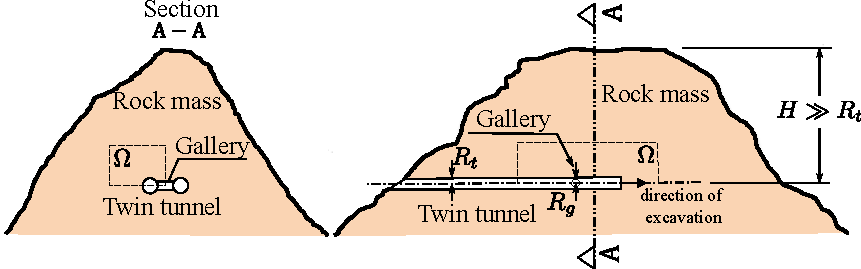
\includegraphics[scale=1]{Domain.pdf}
	\caption{Schematic representation of the twin tunnels geometry problem.}
	\label{domain}
\end{figure}
\FloatBarrier
Within the analyzed material domain, the initial stress state prevailing in the rock mass prior to the tunnel excavation process is defined by constant vertical and horizontal geostatic stress $\sigma_v$ and $\sigma_h$, taking the following form:
\begin{equation} \label{eq:stress0}
	\stress_0 = -\sigma_v \ey \otimes \ey - \sigma_h\left( \onell - \ey \otimes \ey \right)
\end{equation}

where is the upward unit vector parallel to vertical direction. The initial horizontal stress is generally related to the vertical stress by means of the horizontal thrust coefficient $\sigma_h = k_0 \sigma_v$. Starting from the initial configuration of the material system $\Omega$, the processes of excavation (advancing face) and lining placement are simulated by means of the “activation/deactivation” technique [\citenum{bernaud1995}, \citenum{bernaud2009}, \citenum{maghous2012}, \citenum{quevedo2022}].


The geometry material domain $\Omega$ considered for the finite element simulations, including tunnelling and deformation analysis, is defined by a parallelepiped volume of dimensions $\left(L_1+L_2 \right ) \times L_3 \times d_3$ (Fig. 5). Owing to the symmetry of the problem, only the material domain $\left\{x \le 0, y \ge 0\right\}$   is considered for F.E discretization and analysis. Referring to the notations of Fig.~\ref{Mesh1}, $d_1$ is the distance between the axes of longitudinal tunnels, $L_2$  represents the total length  along longitudinal direction $\ez$ of the cylindrical  volume to be excavated that is  considered in the numerical simulation, $d_3$ is the thickness along vertical direction $\ey$ of material domain $\Omega$, $L_1$ stands for the length of unexcavated region after total excavation process, $L_3$ is the total length along transversal direction $\ex$ of discretized material domain, $d_2$ characterizes the location of the circular transverse axis gallery that intersects the  longitudinal tunnel at $z = L_1+d_2$. The length of the excavation step adopted  will be denoted by $L_{pt}$. The finite element model including geometrical discretization and boundary conditions is illustrated in Fig.~\ref{Mesh1}. The mesh used in the simulations consists of $119740$, $182470$ or $221104$ total elements (hexahedra and tetrahedra), depending on the value of spacing between longitudinal tunnels. To increase the accuracy of the model predictions in the intersection zone, the region surrounding the transverse gallery (including part of the longitudinal tunnel) is discretized by means 10-node quadratic tetrahedral elements, whereas 8-node trilinear hexahedral elements are used for the remaining part of the structure.   Furthermore, a refined meshing is used for discretizing the zones surrounding the longitudinal and transverse gallery. These zones whose mechanical state is significantly affected by the tunnelling process are indicated by light gray color in Fig.~\ref{Mesh1}.
\begin{figure}[h!]
	\centering
	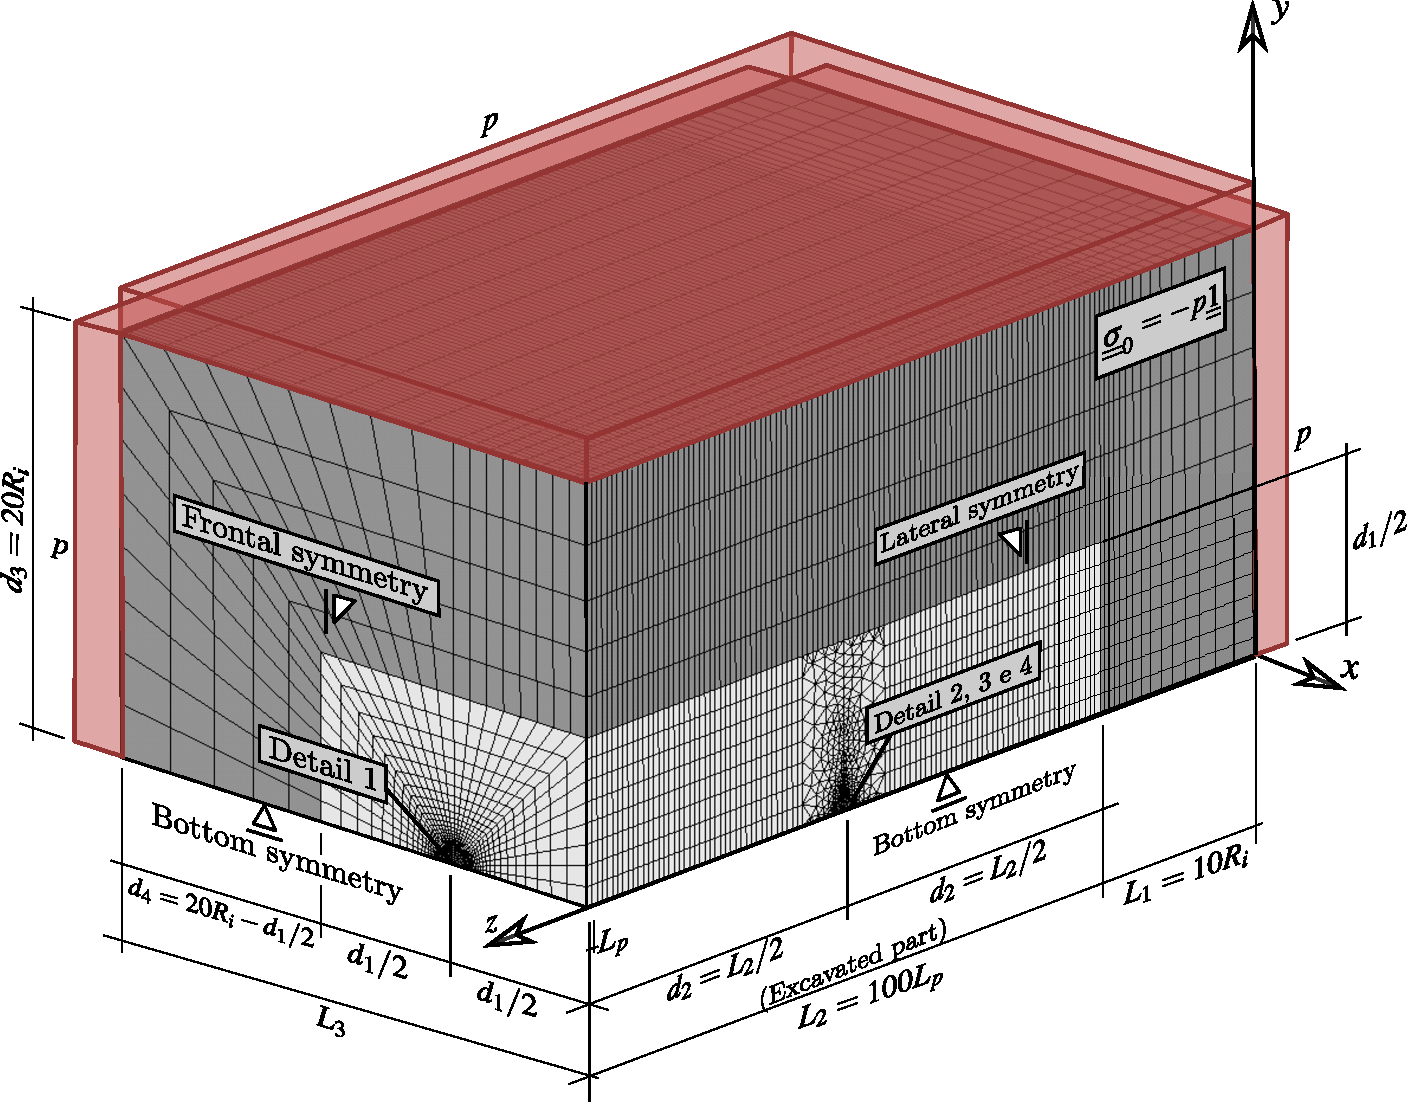
\includegraphics[scale=0.5]{Mesh1.pdf}
	\caption{Mesh, dimensions and boundary conditions of the 3D twin tunnel domain.}
	\label{Mesh1}
\end{figure}

Figures \ref{Mesh2} to \ref{Mesh6} display some details regarding the geometry and F.E discretization of the structure. Fig.~\ref{Mesh2} presents some details of the longitudinal tunnel cross-section in a $xy$ plane, together with the layer of concrete lining (in sky blue color), parameter $e_t$ being the thickness of the lining. Installation of the lining (shotcrete or precast concrete) is simulated in the F.E modeling by progressive activation of the corresponding elements, which consists in assigning to these elements the concrete mechanical properties.
\begin{figure}[h!]
	\centering
	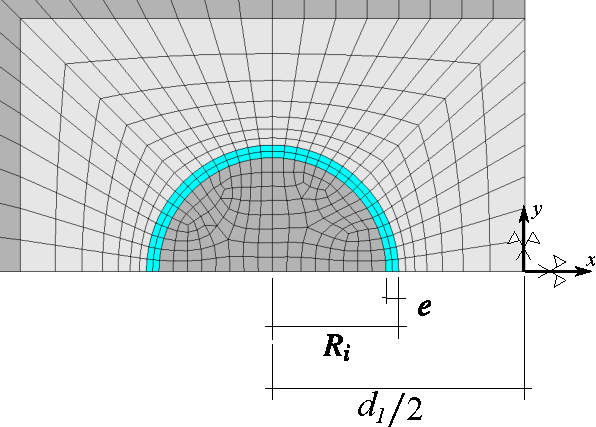
\includegraphics[scale=0.8]{Mesh2.pdf}
	\caption{Detail 1 - Mesh in longitudinal tunnel cross-section with spacing $d_1=4R_t$.}
	\label{Mesh2}
\end{figure}
\FloatBarrier

An important issue investigated in this work is the influence of the spacing $d_1$ between twin tunnels on their convergence. Fig.~\ref{Mesh3} and Fig.~\ref{Mesh4} illustrate the spatial discretization of the gallery region as well as of the connection with the longitudinal tunnel. Three values shall be considered for the spacing $d_1$ in the numerical simulations, namely  $d_1 = 16R_t, 8R_t$ and $4R_t$. The layer of concrete lining of thickness $e_g$ installed along the gallery wall is indicated by red color in the figures. Without introducing additional modeling restriction and for the sake of simplicity, the value of the gallery radius is fixed to $R_g = 2/3R_t$. The same lining system (same concrete material and layer thickness) is considered for both longitudinal tunnels and gallery. As regards the discretization of the region surrounding the gallery, parameters $d_5$ and $d_1$ define the size in a $yz$ plane of the transition region involving the tetrahedral finite elements. Fig.~\ref{Mesh5} provides a view of the transition region and tunnel/gallery intersection zone.
\begin{figure}[h!]
	\centering
	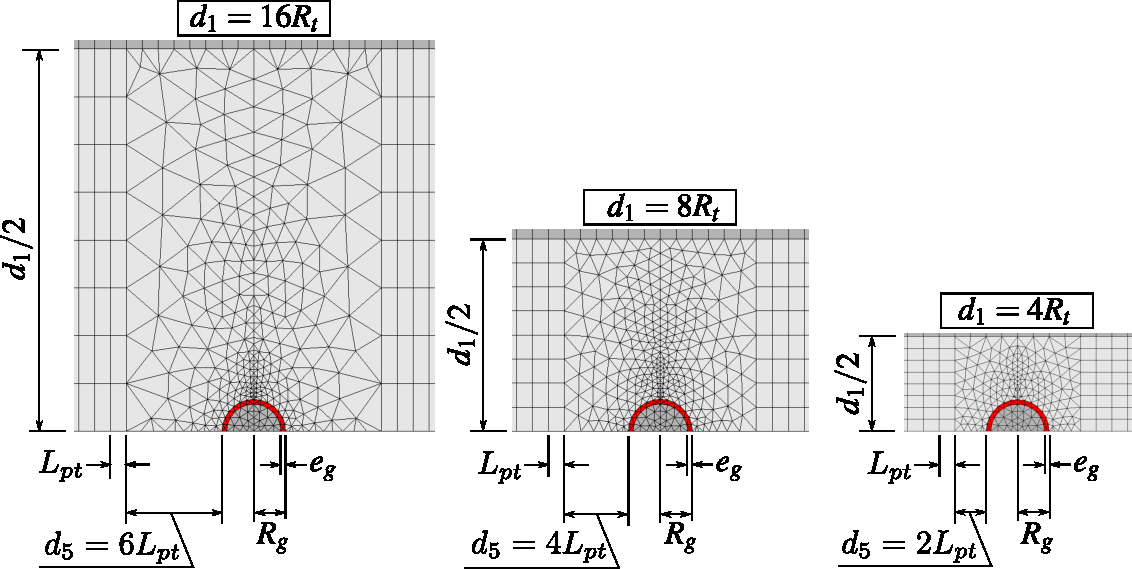
\includegraphics[scale=0.8]{Mesh3.pdf}
	\caption{Geometry and F.E mesh of gallery cross-section for configurations $d_1=16R_t$, $d_1=8R_t$ and $d_1=4R_t$.}
	\label{Mesh3}
\end{figure}
\begin{figure}[h!]
	\centering
	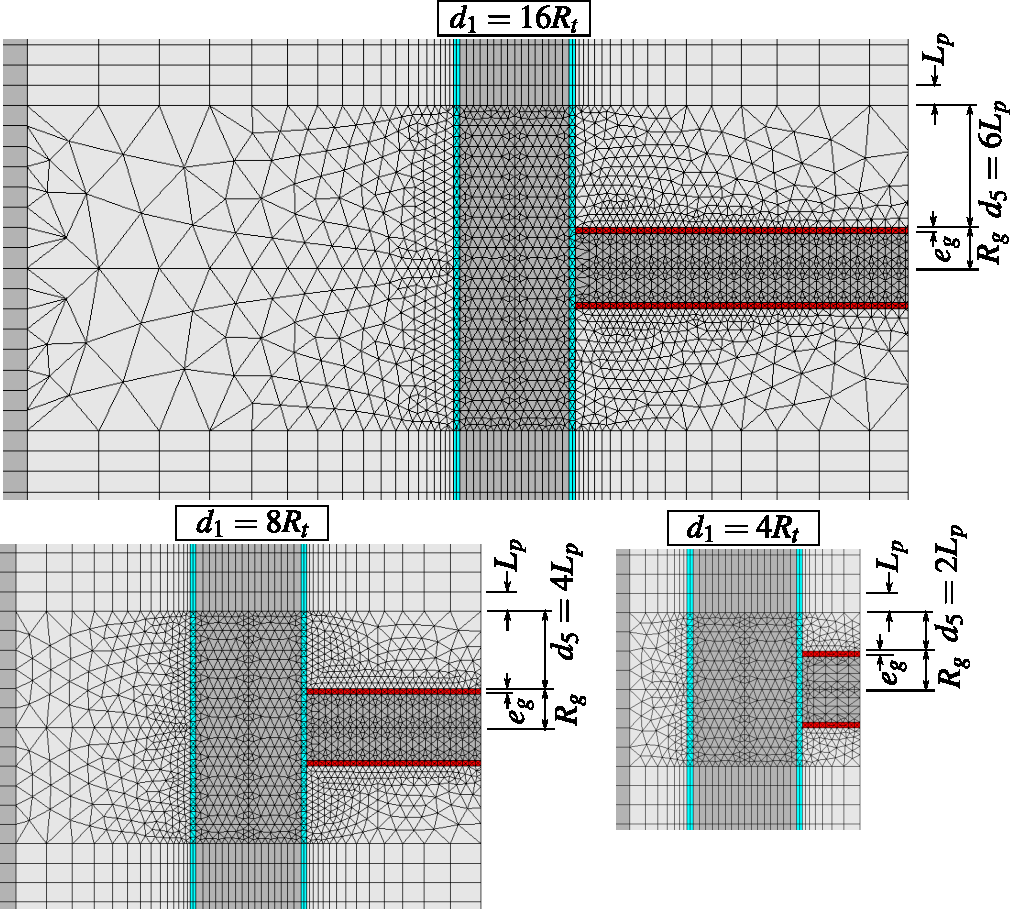
\includegraphics[scale=0.6]{Mesh4.pdf}
	\caption{Views of longitudinal tunnel and gallery in the symmetry plane $y=0$ for configurations $d_1=16R_t$, $d_1=8R_t$ and $d_1=4R_t$.}
	\label{Mesh4}
\end{figure}
\begin{figure}[h!]
	\centering
	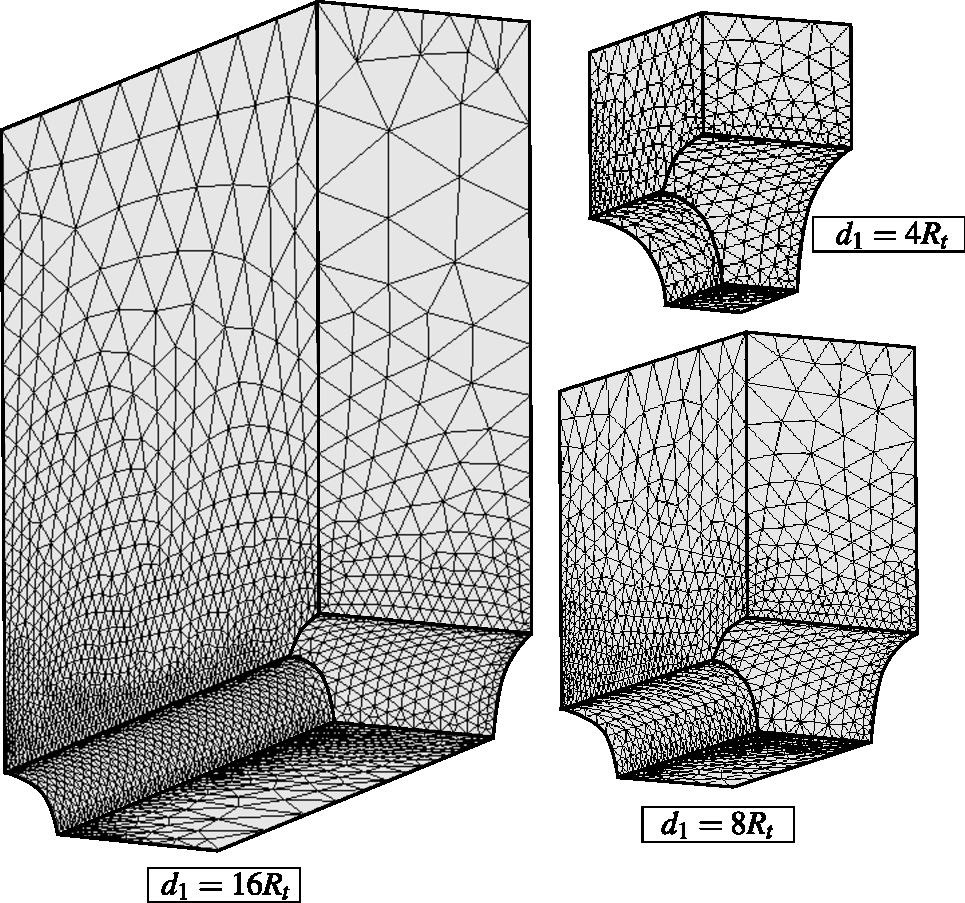
\includegraphics[scale=0.6]{Mesh5.pdf}
	\caption{View of the transition and tunnel/gallery intersection zones for configurations $d_1=16R_t$, $d_1=8R_t$ and $d_1=4R_t$.}
	\label{Mesh5}
\end{figure}
\FloatBarrier

Finally, Fig.~\ref{Mesh6} presents the F.E mesh used for the layer of concrete lining in both the longitudinal layer (in sky blue color) and the gallery (in red color) for the three configurations $d_1=16R_t$, $d_1=8R_t$ and $d_1=4R_t$, with specific details on the junction region of the gallery and the longitudinal tunnel. For the illustration purposes, symmetry with respect to plane $y = 0$ has been used to complete the geometry representation of each configuration. It is emphasized that the tetrahedral elements used for the discretization of the region surrounding the transverse gallery exactly fits excavation steps (elements removal or deactivation).

\begin{figure}[h!]
	\centering
	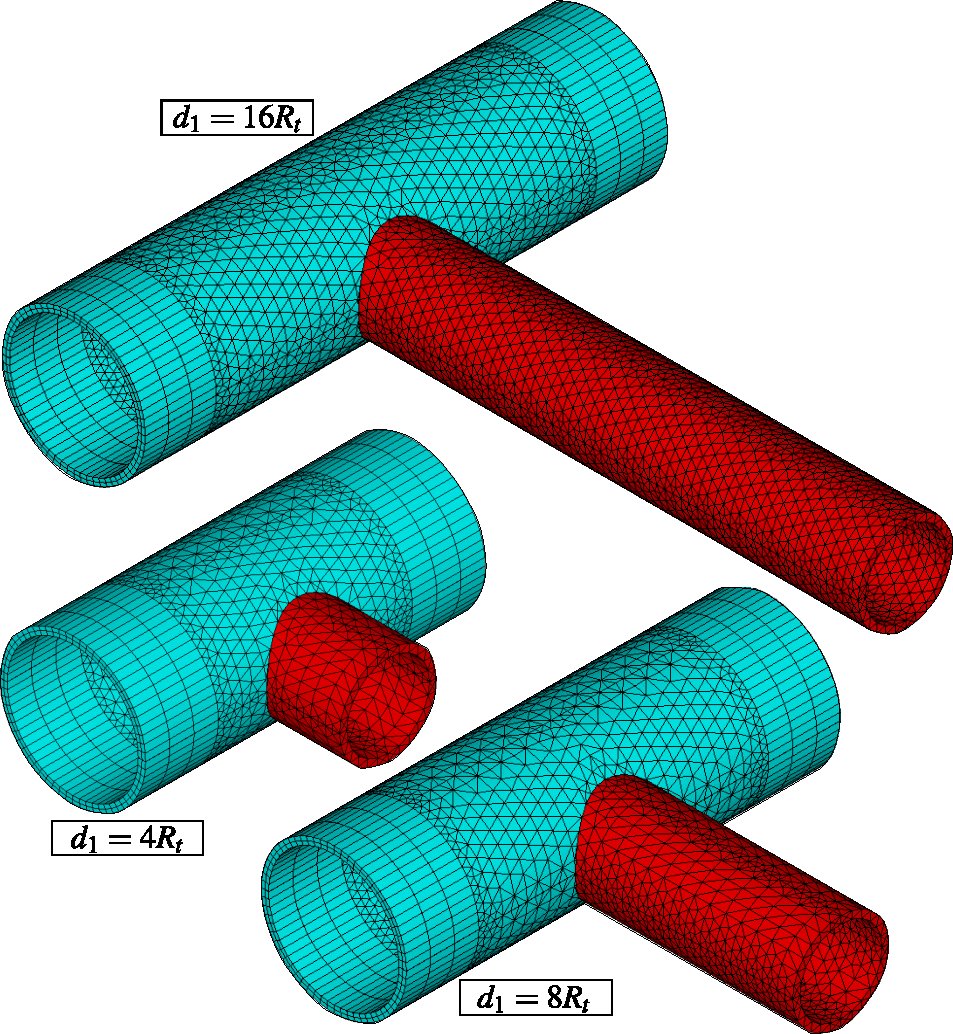
\includegraphics[scale=0.6]{Mesh6.pdf}
	\caption{Isometric view of the lining at the intersection for $d_1=16R_t$, $d_1=8R_t$ and $d_1=4R_t$ - expansion of symmetry in the $xz$ plane.}
	\label{Mesh6}
\end{figure}
\FloatBarrier

As mentioned previously, the tunnelling process, including the excavation steps and lining installation, is simulated resorting to the activation-deactivation method. Each excavation step is modeled by deactivation of the corresponding elements (the elements stiffness is reduced by a factor $1E8$), whereas installation of elements of lining at a distance $d_{0t}$ from the excavation face (unlined length) is achieved through activation of the corresponding elements by assigning them concrete properties. The F.E solution of the time-dependent problem is performed for each excavation step associated with time interval $t_p = L_p/V_p$, where $L_{pt}$ represents the length of the excavation step and $V_{pt}$ is the speed of the excavation face. Fig. 11 schematically displays the consecutive phases of excavation process. In this Figure, $n_p$ is the total number of excavation steps and $n_{pig}$ represents the number of longitudinal tunnel excavation steps prior to gallery excavation. After achievement of the $n_{pig}$ excavation steps, the excavation of the gallery is initiated starting from the longitudinal tunnel wall. Referring to the notation of Fig. 11,  $L_{pg}$ is the considered step length for the gallery excavation, $V_{pg}$ is the speed of the gallery excavation, and $d_{0g}$ is the unlined length of the gallery. Each gallery excavation step is associated with time interval $t_{pg} = V_{pg}/L_{pg}$. After the gallery excavation is completed, we proceed to further excavation steps of the longitudinal tunnel. 

For the sake of clearness, the main parameters defining the geometry domain as well as and excavation process and lining installation are summarized in Table~\ref{table1}. 
\begin{figure}[h!]
	\centering
	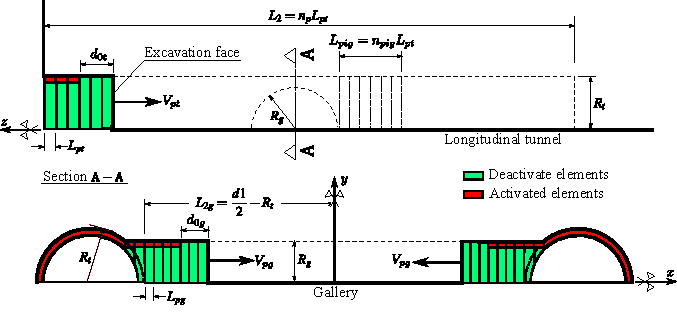
\includegraphics[scale=1.3]{Diagram of excavations.pdf}
	\caption{Schematic representation of the excavation process.}
	\label{Diagram of excavations}
\end{figure}
\FloatBarrier
\begin{table}
	\caption{Parameters related to the geometry of the domain, excavation and installation of the lining.}
	\label{table1}
	\centering
	%\small
	\renewcommand{\arraystretch}{1.25}
	\begin{tabular}{c c c c}
		\hline
		\multicolumn{1}{c}{PARAMETERS} &
		\multicolumn{1}{c}{SYMBOL} &
		\multicolumn{1}{c}{UNIT} &
		\multicolumn{1}{c}{VALUES} \\
		\hline
		\multicolumn{4}{c}{Longitudinal tunnels} \\
		\hline
		Radius of the longitudinal tunnel & $R_t$ & m & $R_t$ \\
		Thickness of the lining & $e_t$ & m & $0.1R_t$ \\
		Step length of the excavation process & $L_{pt}$ & m & $1/3R_t$ \\
		Unlined length & $d_{0t}$ & m & $2L_{pt}$ \\
		Speed of the excavation face & $V_{pt}$ & m/day & $12.5$ \\
		Excavation step time & $t_p$ & day & $L_{pt}/V_{pt}$ \\
		\hline
		\multicolumn{4}{c}{Gallery} \\
		\hline
		Radius of the gallery & $R_{g}$ & m & $2/3R_t$ \\
		Thickness of the concrete lining & $e_g$ & m & $0.1R_t$ \\
		Step length of the excavation process \footnote{1} & $L_{pg}$ & m & $1/3R_g$ \\
		Unlined length & $d_{0g}$ & m & $2L_{pg}$ \\
		Speed of the excavation face & $V_{pg}$ & m/day & $12.5$ \\
		Number of steps that starts gallery excavation & $n_{pig}$ & un & $15$ \\
		\hline
		\multicolumn{4}{c}{Rest of domain} \\
		\hline
		Distance between longitudinal tunnel axes & $d_1$ & m & $4R_t ~8R_t ~16R_t$ \\
		Thickness along vertical direction $\ey$ & $d_3$ & m & $20R_t$ \\
		Length of the unexcavated region & $L_1$ & m & $10R_t$ \\
		Total excavated length & $L_2$ & m & $100L_{pt}$ \\
		Thickness along transversal direction $\ex$ & $L_3$ & m & $20R_t + d_1/2$ \\
		\hline
	\end{tabular}
	\normalsize
	\\ \footnotemark[1]{{\footnotesize Value of $L_{pg}$ is slightly different for the last excavation step to match the gallery lengh.}}
\end{table}
\FloatBarrier
During the tunnel construction phases, the time increment used for the time-dependent analysis is automatically managed by the ANSYS solver. The latter makes use of a semi-implicit scheme for the viscoplasticity solution, together with an automatic time stepping algorithm [\citenum{zienkiewicz1974visco}] in which the time step is defined as a fraction of time $t_p$ for the phases of longitudinal tunnel excavation and as a fraction of $t_{pg}$ for the phases of transverse gallery excavation. Furthermore, distinct time steps are considered for the time-dependent analysis during tunnelling process and post-excavation stage. After complete tunnel construction phases, the analysis is carried out for a period of about $3000$ days to assess the time evolving deformation as well as long-term viscous effects on the final equilibrium of the tunnel structure. At that respect and in anticipation of the numerical results of the subsequent sections, the characteristic viscoplastic relaxation time [\citenum{simo1998}] is equal to $\bar{\tau} = \eta f_0 / E$ , which is close to $30$ days for model data of Table~\ref{table2}.

\section{Preliminary numerical simulations and computational model verification}\label{}

This section is aimed at applying the computational modeling to simulate deformation and stress in two academic twin tunnels configurations. The numerical results provided in these illustrative applications may be viewed as preliminary verifications of the F.E formulation. The first application refers to unlined twin tunnels excavated in an elastic rock mass, whereas the second application addresses the situation of unlined twin tunnels excavated in an elastoplastic medium.

\subsection{Unlined twin tunnels in elastic medium}

In the context of plane strain conditions, Guo et al. [\citenum{GUO2021}] addressed the configuration of deep twin tunnels excavated in a homogeneous elastic medium in which prevails a hydrostatic initial stress distribution. The authors formulated approximate analytical solutions for the stress distribution establishing far behind the face, which are induced in the rock mass by the excavation of two parallel circular tunnels. The model geometry of the twin circular tunnels as well as loading associated with initial hydrostatic stress (i.e., $\sigma_h = \sigma_v$) are displayed in Fig.~\ref{GUO_FIG0}.

Simulation of the problem has been addressed by means of the 3D finite element model and the numerical results obtained for the stress distribution far behind the faces of the twin tunnel shall be compared to the analytical stress solution derived by Guo et al. [\citenum{GUO2021}] in the framework of plane strain conditions. The simulations have been performed taking advantage of symmetry with respect to the midplane between twin tunnels and considering the following model data: tunnel radius $R_t = 4$ m, rock Young modulus $E = 500$ MPa and Poisson ratio $\nu = 0.23$, isotropic initial stresses of $\sigma_v = \sigma_h = 2.2$ MPa.
\begin{figure}[h!]
	\centering
	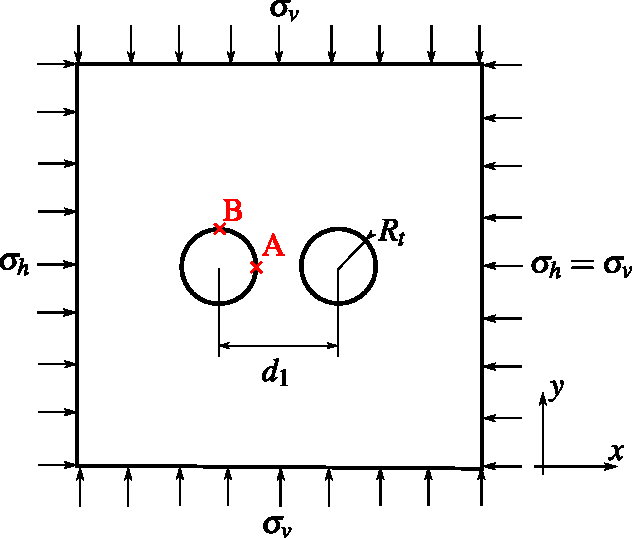
\includegraphics[scale=0.7]{GUO_FIG0.pdf}
	\caption{Geometry model and loading mode of the twin circular tunnels studied in Guo et al. [\citenum{GUO2021}].}
	\label{GUO_FIG0}
\end{figure}
\FloatBarrier

Denoting by $u_y$ the displacement component following the  $y$-axis, Fig.~\ref{Convergence Profiles in B} displays the convergence curves $U_B = -u_y(B)/R_t$ that characterize the inward movement at the tunnel roof $B(x=-d_1/2,y=R_t,z)$ as a function of normalized longitudinal distance to the tunnel face. Several values of normalized distances between the twin tunnels axes $d_1/2R_t$ have been investigated, and the configuration of single tunnel may be viewed as the limiting case $d_1/2R_t \gg 1$. It is recalled that in the latter configuration, the convergence far from the tunnel face that is obtained from an elastic analysis reads $U = \sigma_v(1+\nu)/E$. As expected, this figure indicates that the closer the longitudinal tunnels, the greater the convergence at the roof.
\begin{figure}[h!]
	\centering
	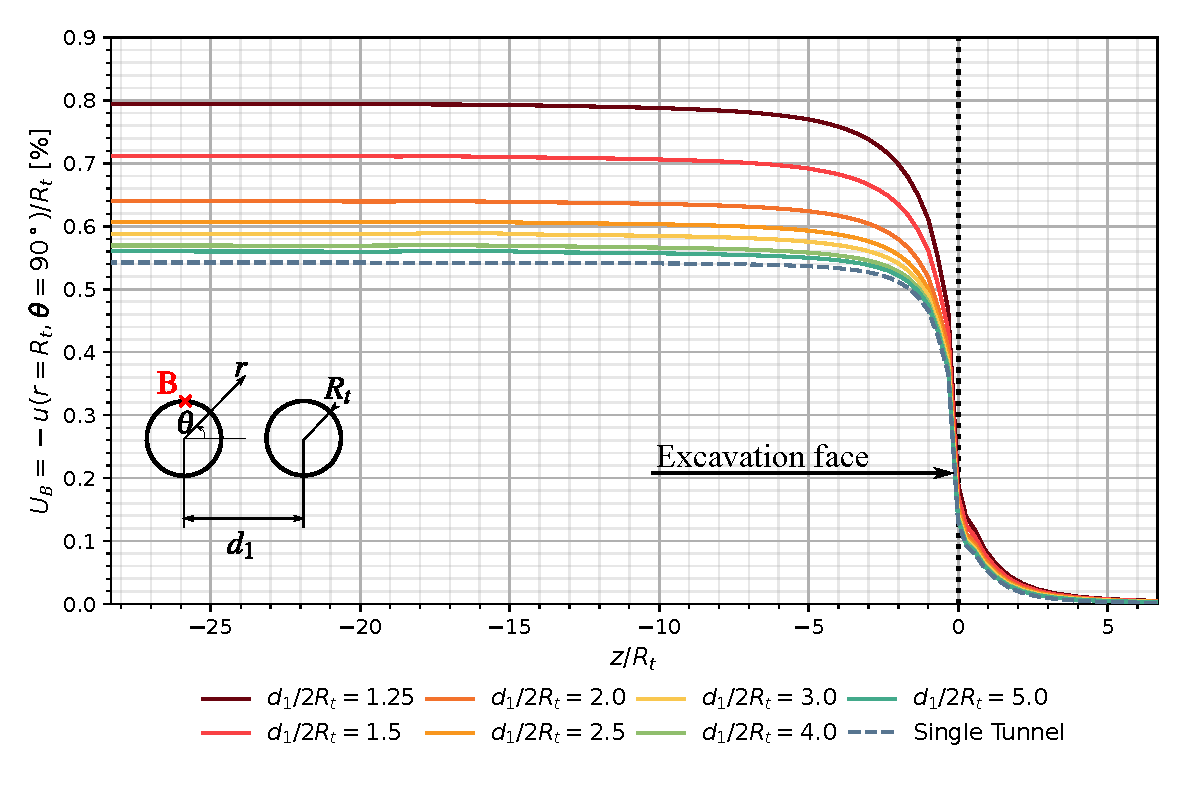
\includegraphics[scale=0.65]{Convergence Profiles in B.pdf}
	\caption{Convergence profiles at the tunnel roof (point B).}
	\label{Convergence Profiles in B}
\end{figure}
\FloatBarrier

The tunnel deformation anisotropy induced by the twin tunnels proximity is illustrated in Fig.~\ref{Relationship between convergence in B and A}, which plots the ratio $U_B/U_A = u_y(B)/u_x(A)$ between the vertical displacement $u_y$ at the roof B and the horizontal displacement $u_x$ at the side wall  $A(x=-d_1/2+R_t, y = 0, z)$. The results shown in this figure refer to a tunnel section located far behind the face at normalized distance $z/R_t = -25$. They emphasize the significative tunnel ovalization induced by the proximity of twin tunnel as the distance $d_1/2R_t$ decreases. 

\begin{figure}[h!]
	\centering
	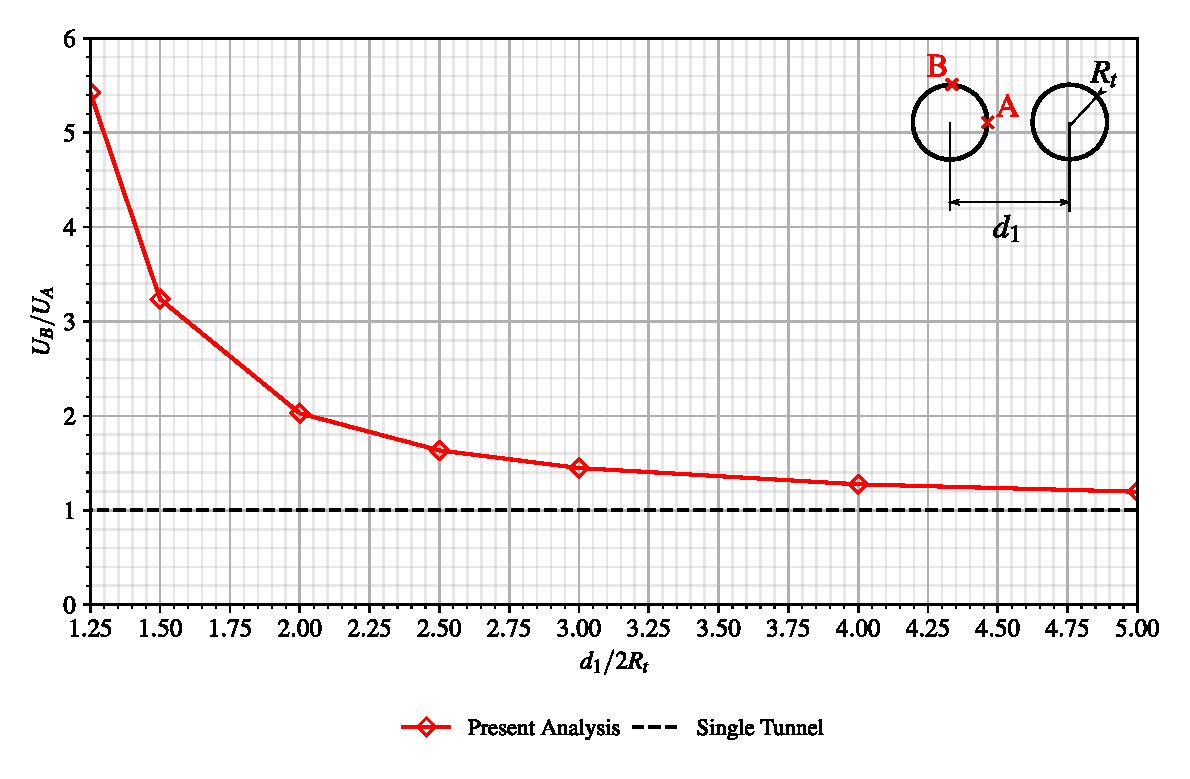
\includegraphics[scale=0.65]{Relationship between Convergence in B and A.pdf}
	\caption{Illustration of the tunnel wall deformation anisotropy induced by twin tunnels proximity.}
	\label{Relationship between convergence in B and A}
\end{figure}
\FloatBarrier

The stress distribution prevailing far from the tunnel face that were obtained from the 3D numerical simulations are compared in Fig.~\ref{Tangencial stress concentration factor in A} to the stress solutions derived analytically and numerically in Guo et al. [\citenum{GUO2021}]. In this figure, the tangential stress concentration factor $\sigma_{yy}/\sigma_v$ computed at the side wall $A$ is plotted for several values of the normalized twin tunnels distance. The results of the theoretical solution to a plate containing two circular holes of equal size presented in Ling et al. [\citenum{ling1948}] are also reported in Fig.~\ref{Tangencial stress concentration factor in A}. It is observed that the results of the 3D finite element simulations correspond to a tunnel section located at normalized distance $z/R_t = -25$ from the face, which is considered sufficient for the plane strain conditions to establish. Interestingly, the tangential stress concentration obtained for a deep single tunnel under plane strain condition simply reads $\sigma_{yy}/\sigma_v = 2$. Although the overall agreement observed between the different predictions, it appears from the comparison that the approximate analytical stress solution provided in [\citenum{GUO2021}] slightly overestimates the tangential stress computed at point A as the value of distance $d_1/2R_t$  increases.

\begin{figure}[h!]
	\centering
	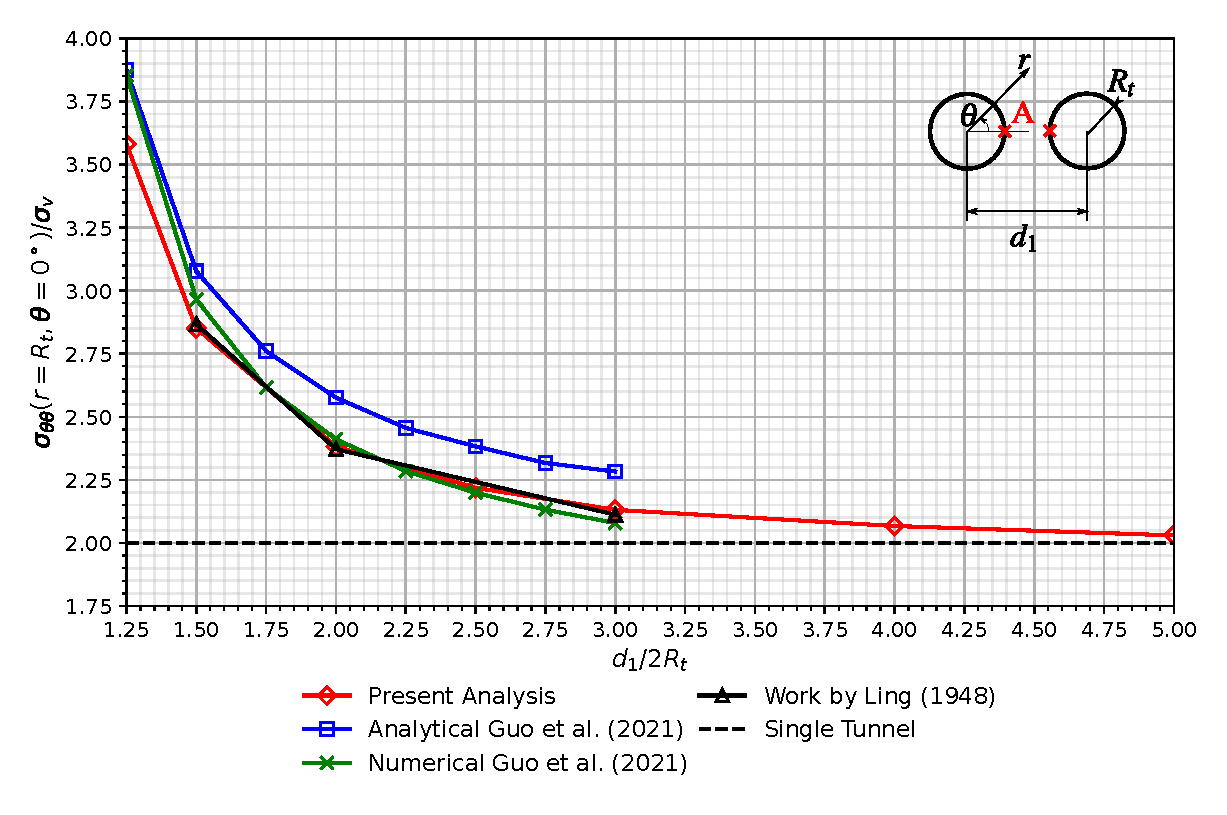
\includegraphics[scale=0.65]{Tangencial stress concentration factor in A.pdf}
	\caption{Tangential stress concentration factor at the side wall A versus twin tunnels distance $d_1/2R_t$.}
	\label{Tangencial stress concentration factor in A}
\end{figure}
\FloatBarrier

Finally, Fig.~\ref{GUO_FIG1} displays the distribution of tangential (orthoradial) stress $\sigma_{\theta \theta}$ around the tunnel boundary $\left\{r = R_t, 0 \le \theta \le \pi\right\}$ considering $d_1/2R_t = 1.5$. The predictions of stress component $\sigma_{\theta \theta}$ obtained from the 3D finite element simulations far behind the tunnel face are shown together with the strain plane solutions derived analytically in [\citenum{GUO2021}], emphasizing the ability of the computational model to accurately capture the effect of tunnels proximity on stress distribution.

\begin{figure}[h!]
	\centering
	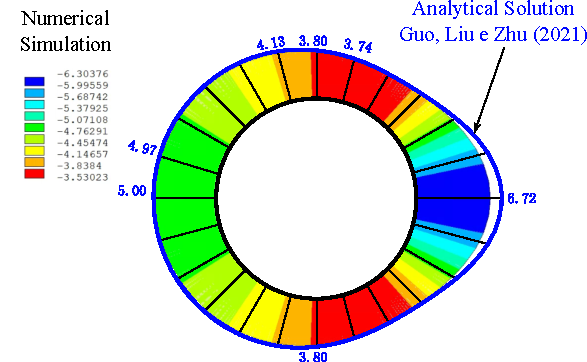
\includegraphics[scale=1]{GUO_FIG1.pdf}
	\caption{Distribution of tangential stress $\sigma_{\theta \theta}$ around the tunnel wall  prevailing far behind the tunnel face (twin tunnels distance $d_1/2R_t = 1.5$).}
	\label{GUO_FIG1}
\end{figure}
\FloatBarrier
Keeping in mind it addresses only an academic configuration, the results provided in this section may be viewed as a first preliminary verification of the accuracy of the computational model formulated for the mechanical interaction in deep twin tunnels.

\subsection{Unlined twin tunnels in elastoplastic medium}\label{}


In the analysis developed by Ma et al. [\citenum{MA2020}], an approximate analytical solution has been formulated for the stresses and the plastic zone boundary around deep twin circular tunnels excavated in a homogeneous elastoplastic medium. The approach carried out under the assumption of plane strain condition makes use of the conformal transformation in the complex variable method to transform the solution of the elastic-plastic interfaces into the determination of the mapping function coefficients.

The geometry model and boundary loading conditions associated with the initial stress state are the same as depicted Fig.~\ref{GUO_FIG0}. Unlike the configuration studied in the preceding section, anisotropic initial stress distributions defined by $\sigma_h \neq \sigma_v$ shall be considered in the present analysis. As regards the rock constitutive model, an elastic-perfectly plastic behavior defined by a Mohr-Coulomb criterion with associated plastic flow rule has been adopted in the study.  Furthermore, the formulation of stress solution for twin tunnels configuration was based on the premise that the plastic zone around each tunnel completely encloses the tunnel edge and the two plastic zones are not connected.

For the comparison purposes, numerical simulations are carried out by means of the 3D finite element model with the aim to investigate the effect of twin tunnels proximity on the tunnel wall deformation. The following model data has been considered in the F.E simulations: tunnel radius $R_t = 1$ m, rock Young modulus $E = 20$ GPa, Poisson ratio $\nu =$ 0.3, friction angle $\phi = 30^\circ$, cohesion $c = 5$ MPa or $2.5$ MPa, initial vertical stress $\sigma_v =30$ MPa or $40$ MPa, initial horizontal stress $\sigma_h = 30$ MPa or $40$ MPa. The simulation took advantage symmetry with respect to the midplane between the twin tunnels has been used for in the F.E discretization model.

Similarly to the analysis developed in the preceding section, the convergence curves $U_B=-u_y(B)/R_t$, which reflects the inward movement at the tunnel roof $B(x=-d_1/2, y=R_t, z)$, is depicted in Fig.~\ref{MA_convergence_profile_B} as a function of normalized longitudinal distance to the tunnel face. Several values of normalized distances between the twin tunnels axes $d_1/2R_t$ have been investigated, together with the reference configuration of single tunnel, the latter being viewed as the limiting case $d_1/2R_t \gg 1$. As it could be expected from such simulations, this figure indicates that the proximity of tunnels significantly increases the convergence at the tunnel roof for small values, say $d_1/2R_t < 2$, of twin tunnel spacing. However, this effect rapidly become negligible as soon as the tunnel spacing increases.

\begin{figure}[h!]
	\centering
	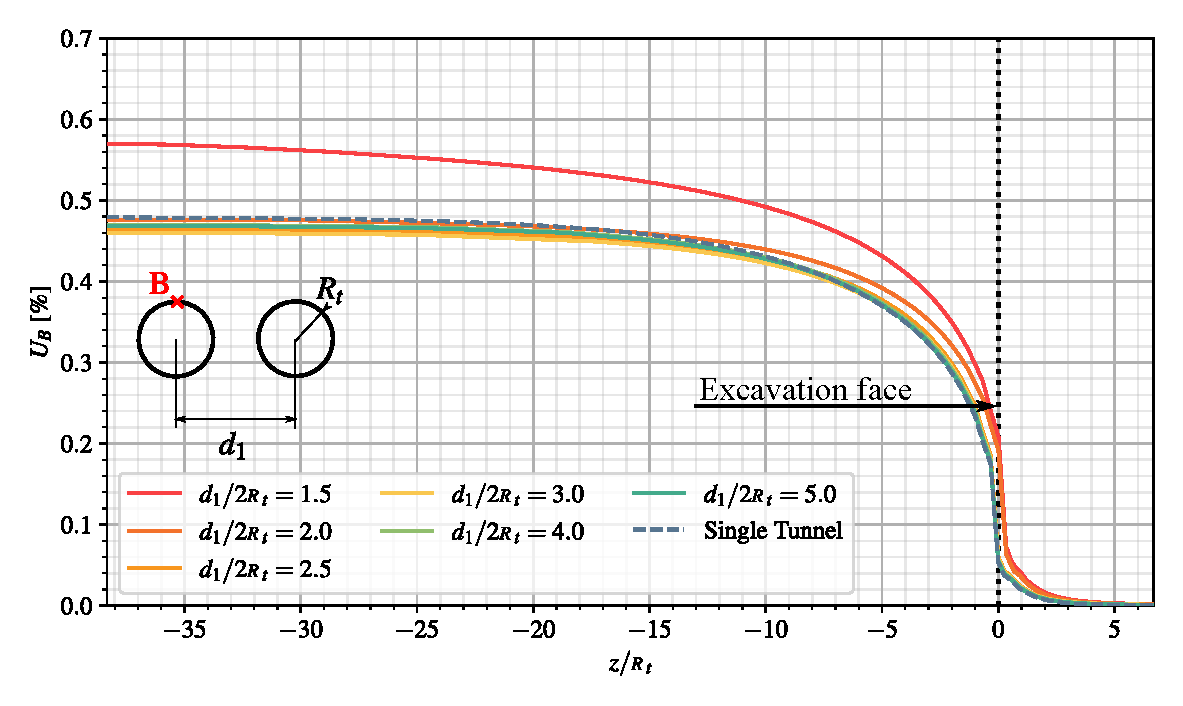
\includegraphics[scale=0.65]{MA_Convergence Profiles in B.pdf}
	\caption{Convergence profiles at the tunnel roof (point B): $c=5$ MPa, $\sigma_v = \sigma_h = 30$ MPa.}
	\label{MA_convergence_profile_B}
\end{figure}
\FloatBarrier

An important feature of the twin tunnels deformation is related to the anisotropy induced by the mutual interaction as the normalized tunnel spacing $d_1/2R_t$ decreases. In that respect, anisotropy of tunnel deformation is illustrated in Fig.~\ref{MA_Relationship between convergence in B and A}, which presents the variations of the ratio $U_B/U_A = u_y(B)/u_x(A)$ between the vertical displacement $u_y$ at the roof $B$ and the horizontal displacement $u_x$ at the side wall $A(x =-d_1/2+R_t, y = 0, z)$ as a function of  normalized twin tunnel spacing $d_1/2R_t$. These results refer to a tunnel section located far behind the face at normalized distance $z/R_t = -35$. As observed in the elastic case studied in the preceding section, the proximity of twin tunnels reflected by small values of normalized distance $d_1/2R_t$ is responsible for tunnel ovalization. The magnitude of horizontal displacement at the side wall $A$ is actually larger in than that of vertical displacement at the tunnel roof $B$, thus indicating an ovalization in the vertical direction (i.e., parallel to $y$-axis).

\begin{figure}[h!]
	\centering
	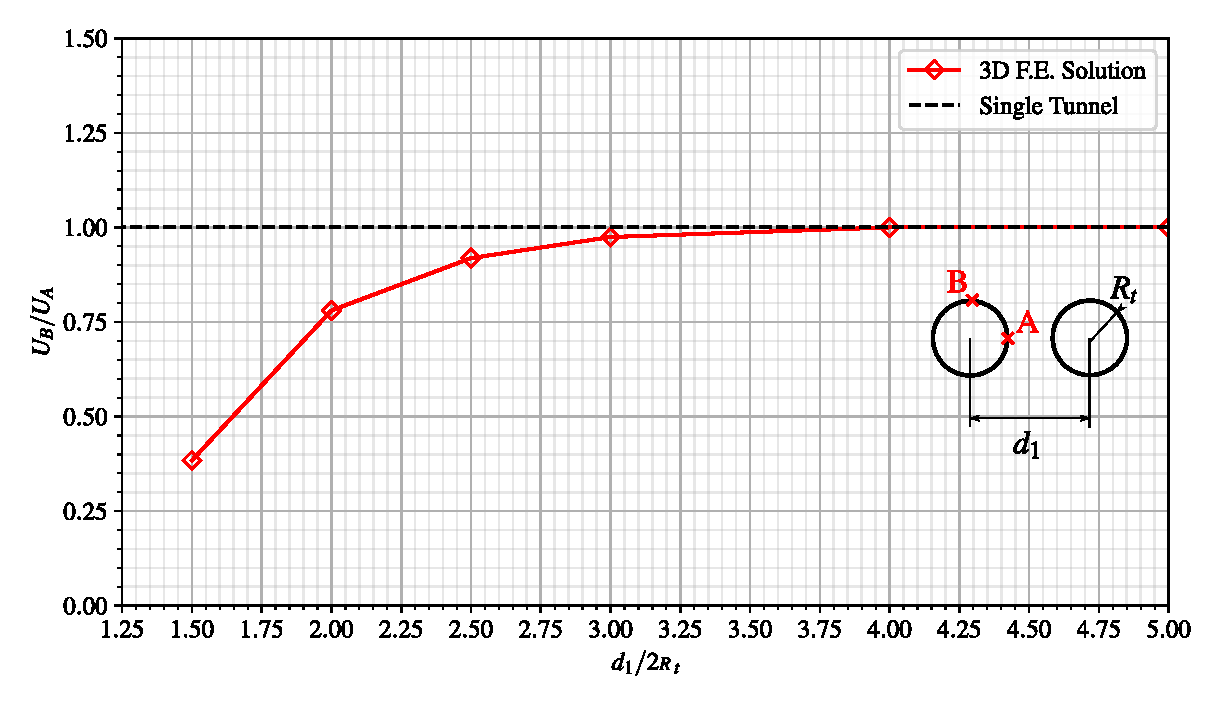
\includegraphics[scale=0.65]{MA_Relationship between Convergence in B and A.pdf}
	\caption{Tunnel wall deformation anisotropy induced by twin tunnels proximity: $c=5$ MPa, $\sigma_v = \sigma_h = 30$ MPa.}
	\label{MA_Relationship between convergence in B and A}
\end{figure}
\FloatBarrier

The stress distribution prevailing far from the tunnel face that were obtained from the 3D numerical simulations are compared in the to the approximate stress solutions derived by Ma et al. [\citenum{MA2020}] within the context of plane strain conditions. Fig.~\ref{MA_FIG1} displays such a comparison in terms of predicted plastic zone surrounding the twin tunnels considering a normalized tunnel spacing of $d_1/2R_t = 2.5$.  Different values have been considered for rock cohesion $c$ and initial stresses $\sigma_v$ and $\sigma_h$. It appears from the latter figure that the finite element modeling produces predictions very similar to those provided in \ref{MA_FIG1}. The results also illustrate that larger plastic zones arise when the cohesion $c$ is smaller.

\begin{figure}[h!]
	\centering
	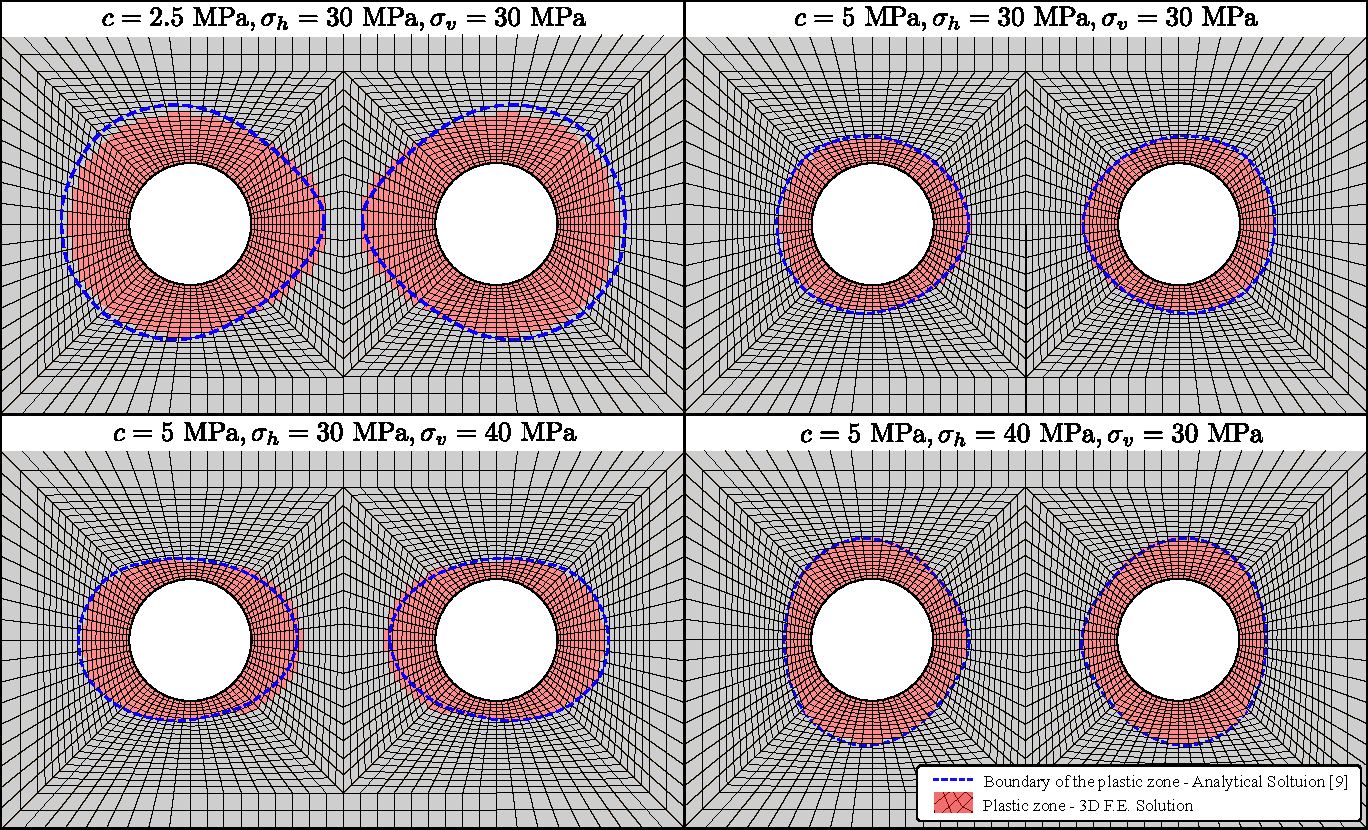
\includegraphics[scale=0.7]{MA_Comparisions_plastic_zones.pdf}
	\caption{The plastic zone extent obtained from the present F.E. simulations and from the stress solution provided in [\citenum{MA2020}].}
	\label{MA_FIG1}
\end{figure}
\FloatBarrier
Further comparisons are shown in Fig.~\ref{MA_stresspaths}, which presents the plots of radial $\sigma_{rr}$, and orthoradial $\sigma_{\theta \theta}$ stress components along three radial paths defined in polar coordinates by $\theta = 45^\circ,~90^\circ \text{~and~} 135^\circ$. It should be pointed out that, although the F.E element simulations make use of the Drucker-Prager yield surface inscribed to the Mohr-Coulomb one (used in the solution of Ma et al. \citenum{MA2020}), the numerical predictions are matching well with the analytical stress solution.

\begin{figure}[h!]
	\centering
	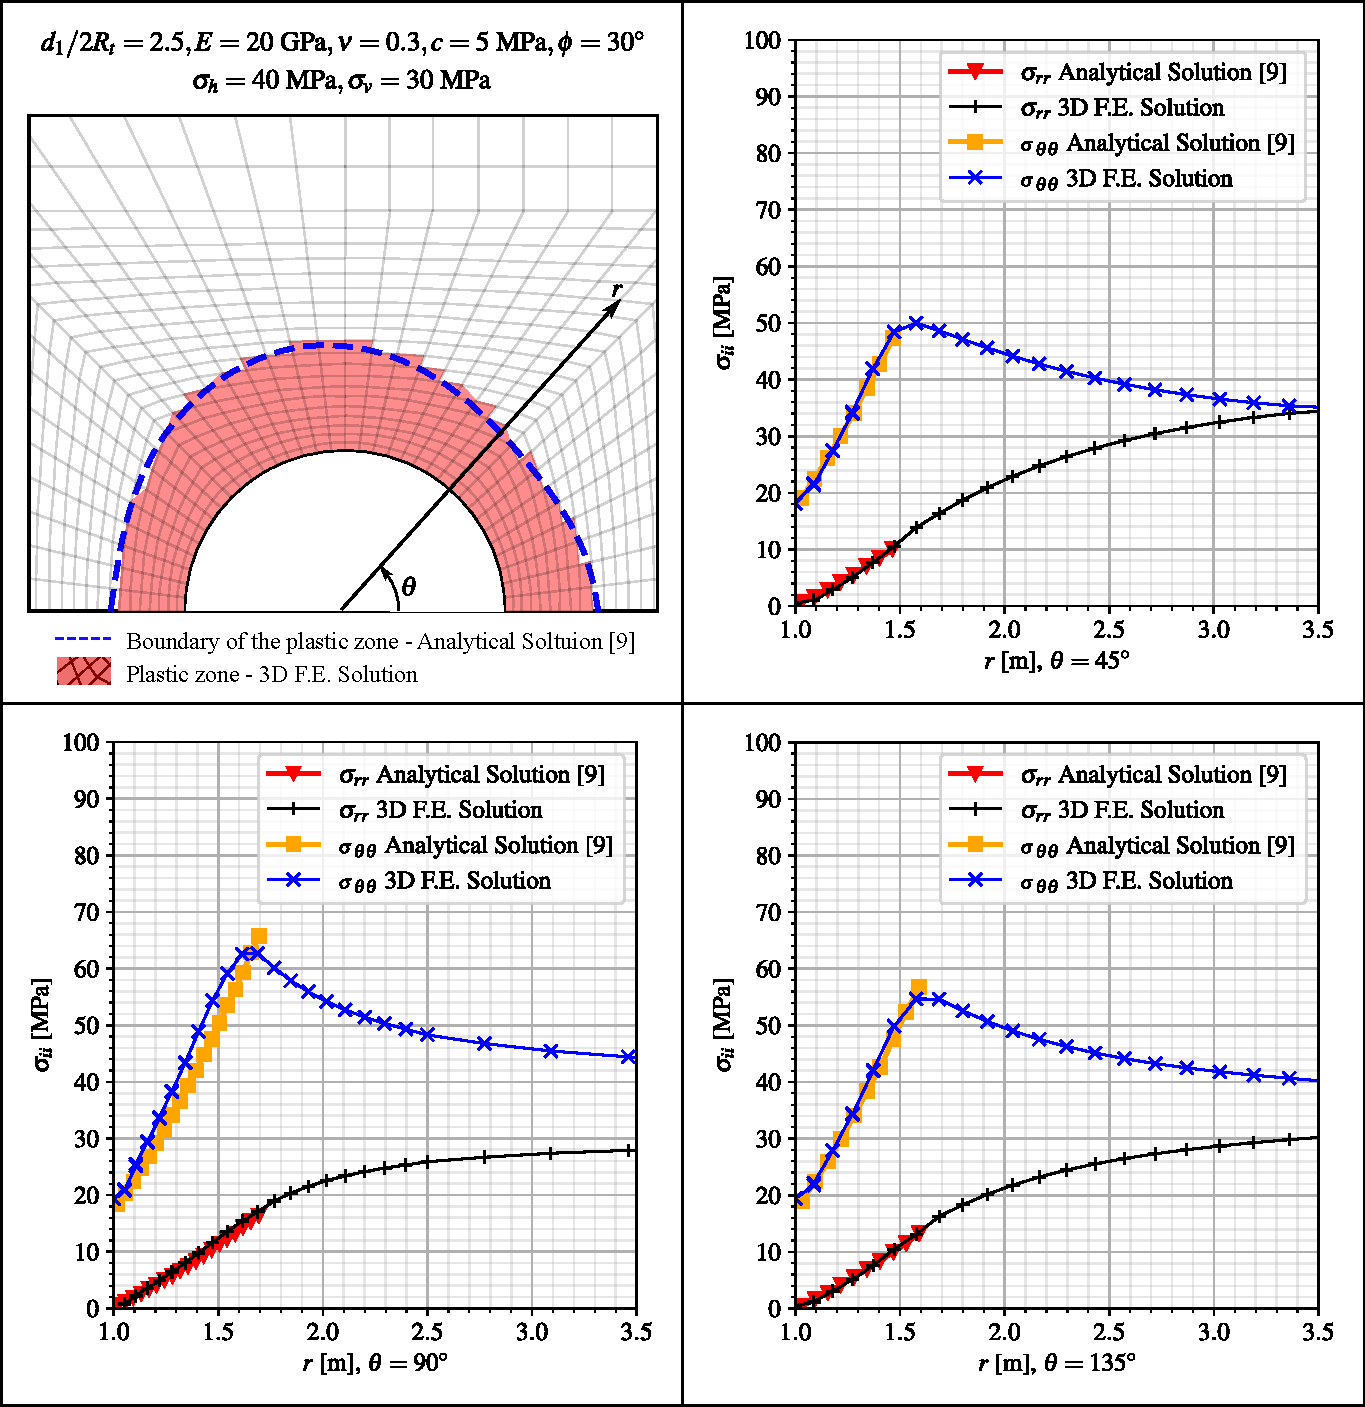
\includegraphics[scale=0.6]{MA_stresspaths.pdf}
	\caption{Distribution of radial and orthoradial stress components along different radial directions: comparison between numerical and analytical predictions.}
	\label{MA_stresspaths}
\end{figure}
\FloatBarrier

\section{Numerical Results and Discussion}\label{}

In this section, the main results obtained from the parametric analysis, considering different constitutive models and distances between the longitudinal tunnels, are presented and discussed. The section is organized as follows: first, the constitutive parameters and observations on the results are presented; next, analyses considering short- and long-term effects, including the impact of ovalization, are discussed; then, long-term analyses focusing solely on viscous models are considered; and finally, the effect of lining stiffness on the evolution of convergence is examined.

\subsection{Constitutive parameters and observations about results}\label{}

The parametric analysis uses the constitutive parameters of the incompressible clay rock mass of the eastern Paris basin (Aisne, France), as detailed in [\citenum{rousset1988}], [\citenum{giraud1993}] and [\citenum{piepi1995}] and summarized in Table~\ref{table2}. The parameter values are derived qualitatively from various triaxial compression tests, including creep tests conducted mainly in undrained conditions. The Aisne clay rocks exhibit high density  (2.01 to 2.57 g/cm$^3$), a low average water content (between 3 to 11\%) and, are characterized by low porosity (typically less then 20\%). Therefore, hydromechanical coupling has minimal significance. The long-term effects primarily stem from material viscosity, with a low proportion attributable to pore pressure redistribution (hydraulic diffusion). Another characteristic is that irreversible deformations are observed in cyclic tests even at small values of axial deformation (less than 0.3\%). Furthermore, for in situ confinement values (approximately 450 m deep), the maximum deviator remains practically constant, suggesting a Tresca-type failure criterion. In the creep tests, the magnitude of delayed deformations is comparable to that observed during instantaneous tests, with a deviatoric stress threshold beyond which creep phenomena initiate. Moreover, the influence of confining pressure on creep phenomena can be disregarded, and comparing both behaviors, instantaneous and delayed, reveals that short-term cohesion exceeds long-term cohesion, with the ratio between these two cohesion values ranging from 1.2 and 2. 

Table~\ref{table2} also presents the constitutive parameters for the lining, based on typical values for reinforced concrete. For the elastic analyses, Young's modulus at 28 days is employed. In the viscoelastic analyses, however, Young's modulus evolves as the lining ages. Each segment of the lining begins aging from the moment it is activated during the construction process. The effect of shrinkage begins at the age of $t_s = 7$ days and creep begin at the age of loading, at $t_0 = 1$ day.

\begin{table}[h!]
	\caption{Constitutive parameters used in the parametric analysis.}
	\label{table2}
	\centering
	%\small
	\renewcommand{\arraystretch}{1.25}
	\begin{tabular}{c c c c}
		\hline
		\multicolumn{1}{c}{PARAMETERS} &
		\multicolumn{1}{c}{SYMBOL} &
		\multicolumn{1}{c}{UNIT} &
		\multicolumn{1}{c}{VALUES} \\
		\hline
		\multicolumn{4}{c}{Constitutive model of rock mass} \\
		\hline
		Young's modulus & $E$ & MPa & $1500$ \\
		Poisson's ratio & $\nu$ & - & $0.49$ \\
		Plastic cohesion & $c$ & MPa & 4$\sqrt{3}/2$ \\
		Plastic friction angle & $\phi$ & $^{\circ}$ & 0 \\
		Viscoplastic cohesion & $c_{vp}$ & MPa & 2$\sqrt{3}/2$ \\
		Viscoplastic friction angle & $\phi_{vp}$ & $^{\circ}$ & 0 \\
		Power law parameter & $n$ & - & 1 \\
		Reference parameter & $f_0$ & MPa & 1 \\
		Viscosity coefficient & $\eta$ & day & $40000$ \\
		\hline
		\multicolumn{4}{c}{Constitutive model of lining} \\
		\hline
		
		Characteristic compressive strength at age of 28 days & $f_{ck}$ & MPa & $20$ \\
		Modulus of elasticity at the age of 28 days & $E_{c_{28}}$ & MPa & $30303$ \\
		Poisson's ratio & $\nu_c$ & - & $0.2$ \\
		
		Coefficient which depends on the type of cement & $s$ & - & $0.2$ \\
		Relative humidity of ambient environment & $RH$ & \% & $70$ \\
		Notional size of member - longitudinal concrete lining & $h_t$ & cm & $0.2111$ \\
		Notional size of member - gallery concrete lining & $h_{g}$ & cm & $0.2176$ \\
		Age of concrete at the beginning of shrinkage & $t_s$ & days & $7$ \\
		Coefficient in shrinkage which depends on the type of cement & $\beta_{sc}$ & - & $8$ \\
		Temperature & $T$ & $^\circ$C & $20$ \\
		Age of concrete at loading & $t_0$ & days & $1$ \\
		\hline
	\end{tabular}
	\normalsize
\end{table}
\FloatBarrier

In this study, an initial hydrostatic stress of $\sigma_v = \sigma_h = 9$ MPa, corresponding to a depth of 450 m, was adopted, simulating the conditions of the rock mass characterization. The study examines the long-term and short-term convergence profiles using various constitutive models for the rock mass (elastic, elastoplastic, and viscoplastic) and the lining (elastic, and viscoelastic), including scenarios without lining. For clarity, Table~\ref{table3} lists the abbreviations used throughout the text and in the results legends. These analyses are conducted for three different distances between the longitudinal tunnels ($d_1 = 4R_t$, $8R_t$, and $16R_t$), using a tunnel radius $R_t=1$ m and an excavation speed of 12.5 m/day. Additional geometric parameters for the domain, excavation, and lining installation are provided in Table~\ref{table1}, with further details discussed in Section~ \ref{section_spatial}.

\FloatBarrier
\begin{table}[h!]
	\caption{Abbreviation to the constitutive models and scenarios.}
	\label{table3}
	\centering
	%\small
	\renewcommand{\arraystretch}{1.25}
	\begin{tabular}{c c}
		\hline
		\multicolumn{1}{c}{DESCRIPTION} &
		\multicolumn{1}{c}{ABBREVIATION} \\
		\hline
		Elastic rock mass & E \\
		Elastoplastic rock mass & EP \\
		Elastoviscoplastic rock mass & VP \\
		Elastoplastic-Viscoplastic rock mass & EPVP \\
		Not lining & NL \\
		Elastic lining & EL \\
		Viscoelastic lining & VEL \\
		Long-term & LT \\
		Final excavation (Short-term) & ST \\
		With Gallery & WG \\
		Not Gallery & NG \\			
		\hline
	\end{tabular}
	\normalsize
\end{table}
\FloatBarrier

Denoting by $u_y$ the displacement component along the y-axis, all the results presented in the following analyses, show the convergence profile $U_B = -u_y(B)/R_t$, which characterize the inward movement of the tunnel roof $B(x = 0, y = R_t, z)$ as a function of the normalized longitudinal distance from the excavation face. In addition, point $C(x=0, y =R_t, z = -25)$ was chosen to denote the equilibrium convergence $U_C$ outside the region of influence of the excavation face and the gallery. When the gallery is present, the highest convergence value, $U_{peak}$ is highlighted at the coordinate where the gallery intersects the longitudinal tunnels $D(x=0, y = R_t, z = L_1+L_2/2)$.

An important observation is that in single tunnels, under rock mass isotropy and hydrostatic initial stress state conditions, the symmetry of the tunnel wall is preserved throughout the excavation process. Thus, the deformed tunnel wall remains circular. On the other hand, one of the effects of the mutual interaction induced by the proximity of the twin tunnels is the loss of symmetry of the deformed tunnel wall. Fig.~\ref{Ovalization effect and monitoring point} presents tunnel roof B and the effect of ovalization due to the proximity of the tunnels. In this context, $U_B$ is not representative of the entire deformation of the tunnel wall.
\begin{figure}[h!]
	\centering
	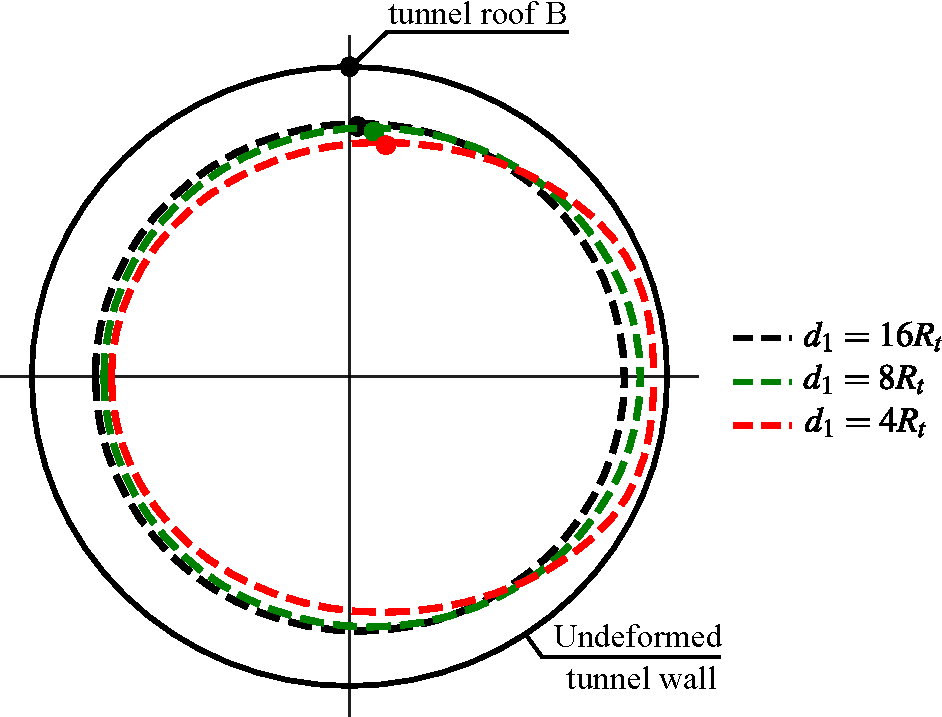
\includegraphics[scale=0.5]{Ovalization effect and monitoring point.pdf}
	\caption{Monitoring point and ovalization effect.}
	\label{Ovalization effect and monitoring point}
\end{figure}
\FloatBarrier

Another important observation regarding the material properties shown in Table~\ref{table2} is that the value adopted for plastic cohesion ($c$) is greater than the value for viscoplastic cohesion ($c_{vp}$): $c$ > $c_{vp}$. This implies that, in the regime of irreversible deformations, the viscoplasticity of the material will be activated first. The generic configurations of the rock mass deformation zones during the excavation process are illustrated in Fig.~\ref{zones}.

\begin{figure}[h!]
	\centering
	\includegraphics[scale=0.6]{zones.pdf}
	\caption{Configurations for the zones with irreversible deformations in the rock mass.}
	\label{zones}
\end{figure}

\subsection{Short and long-term analysis and ovalization effect}\label{}

Figs.~\ref{WG-ST-LT-D1-16RI}, \ref{WG-ST-LT-D1-8RI}, and \ref{WG-ST-LT-D1-4RI} show the convergence profiles of the twin tunnels with gallery (WG) for all the constitutive models of the rock mass (E - blue, EP - yellow, VP - magenta, EPVP - red and green) and the lining (EL and VEL) in the short-term (ST - solid lines) and the long-term (LT - dashed lines), for $d_1 = 16R_t, 8R_t$ and $4R_t$ respectively.
\begin{figure}[h!]
	\centering
	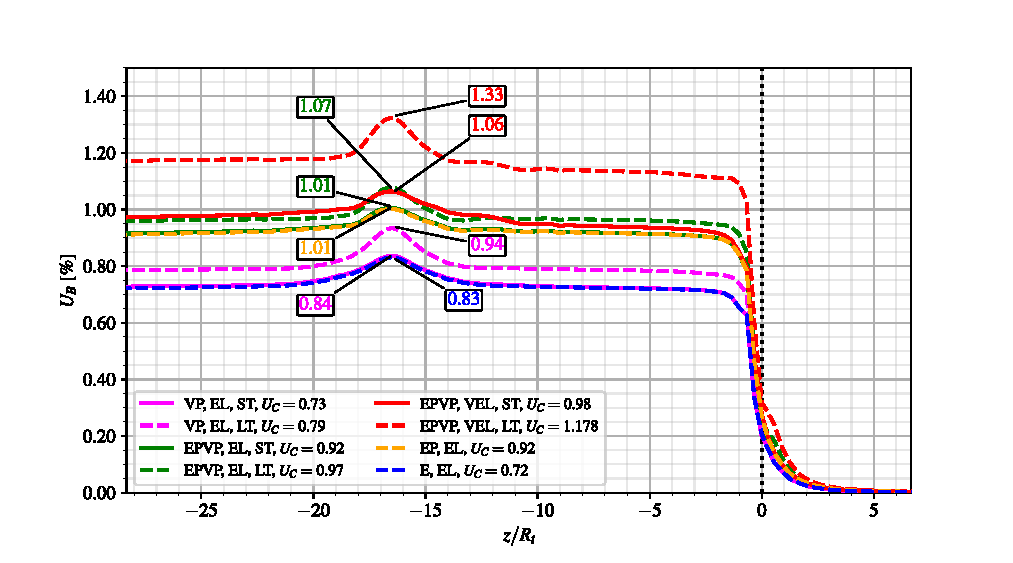
\includegraphics[scale=0.9]{Convergence Profiles - WG_ST_LT - $d_1=16R_i$_anotate.pdf}
	\caption{Convergence Profiles - with gallery (WG), short-term (ST) and long-term (LT) for $d_1 = 16R_t$.}
	\label{WG-ST-LT-D1-16RI}
\end{figure}
\FloatBarrier
\begin{figure}[h!]
	\centering
	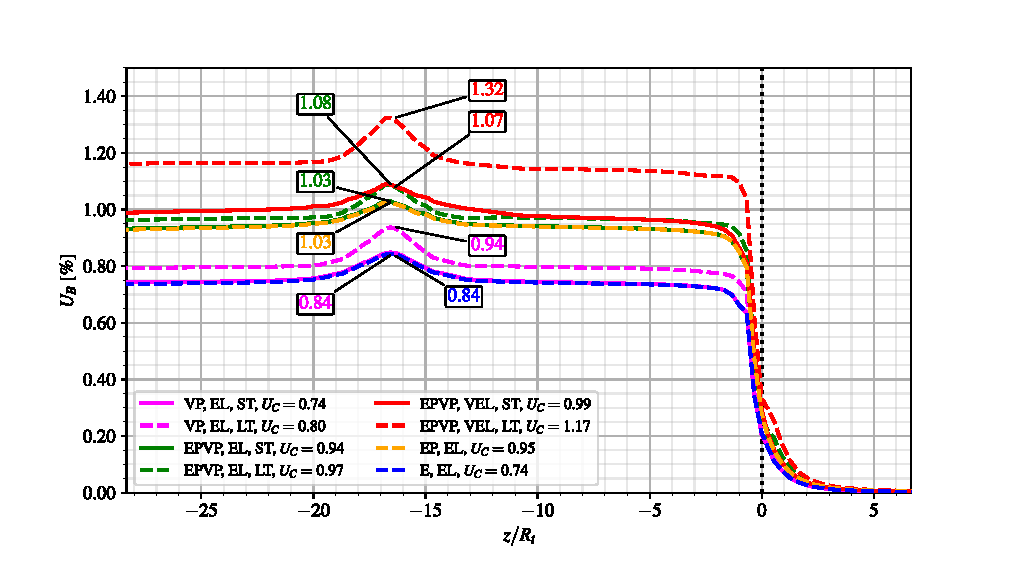
\includegraphics[scale=0.9]{Convergence Profiles - WG_ST_LT - $d_1=8R_i$_anotate.pdf}
	\caption{Convergence Profiles - with gallery (WG), short-term (ST) and long-term (LT) for $d_1 = 8R_t$.}
	\label{WG-ST-LT-D1-8RI}
\end{figure}
\FloatBarrier
\begin{figure}[h!]
	\centering
	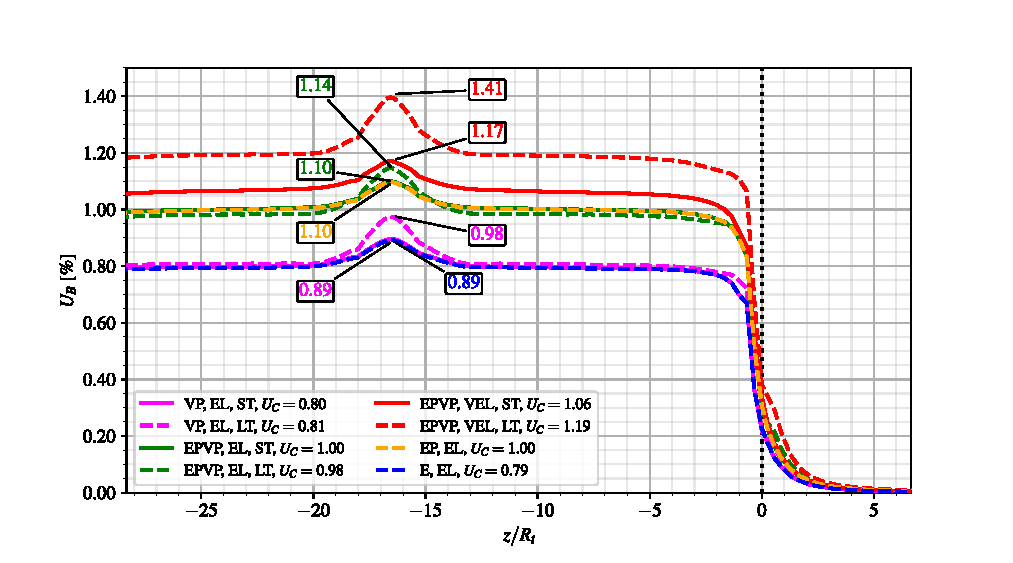
\includegraphics[scale=0.9]{Convergence Profiles - WG_ST_LT - $d_1=4R_i$_anotate.pdf}
	\caption{Convergence Profiles - with gallery (WG), short-term (ST) and long-term (LT) for $d_1 = 4R_t$.}
	\label{WG-ST-LT-D1-4RI}
\end{figure}
\FloatBarrier
In all $d_1$ distances, the convergence profiles of the E-EL (blue dashed line) and the VP-EL (magenta solid line) in the short-term (ST) are equivalent, due to the high excavation speed. The high speed of the excavation and installation of the lining limits the time for the viscous effects to manifest themselves also taking into account the restriction imposed by the stiffness of the lining.

In the short-term (ST), the EPVP-EL model (green solid line) is equivalent to the EP-EL (yellow dashed line) because, although plasticization around the section has already occurred due to excavation, the viscous effects have not yet evolved considerably due to the short time between the start and end of excavation process. However, in the long-term (LT), as convergence continues (dashed green line), differences become apparent. When the rheological effects of the lining are considered, the profile continues to evolve significantly, as seen in the EPVP-VEL model (solid and dashed red lines).

An important aspect is that the stiffness of the elastic lining significantly impeded the evolution of convergence under viscous effects. This is particularly evident in the VP-EL model with $d_1=4R_t$ (solid and dashed magenta line). In this case, the interaction between nearby twin tunnels causes a substantial increase in the value of $U_{C}$ in the short-term (ST). However, the long-term profile (LT) hardly changes, remaining close to the short-term one due to the limitation imposed by the stiffness of the lining.

Another noteworthy aspect is that the EPVP-VEL model with $d_1 = 16R_t$ (red dashed line) has a reduction in $U_{B}$ convergence after 15 excavation steps ($n_{pig}$) from the gallery. This phenomenon is due to the evolving viscous effects of the already-excavated longitudinal tunnel during the gallery excavation. This effect becomes more pronounced with $d_1 = 16R_t$ which spends the longest time excavating the gallery. When the gallery lenght is smaller ($d_1 = 8R_t$ and $4R_t$), the time elapsed is shorter, and this effect is less pronounced.

The effect of ovalization can also be seen in the convergence profile. The EPVP-EL-LT model (green solid line) has a slightly lower convergence than the EPVP-EL-ST (green dashed line) for $d_1 = 4R_t$. The ovalization effect is responsible for the roof's convergence decreasing over time. However, another point in the tunnel wall experiences an increase in convergence. Fig.~\ref{ovalization} illustrates this effect away from the gallery influence region with a single tunnel reference.

\begin{figure}[h!]
	\centering
	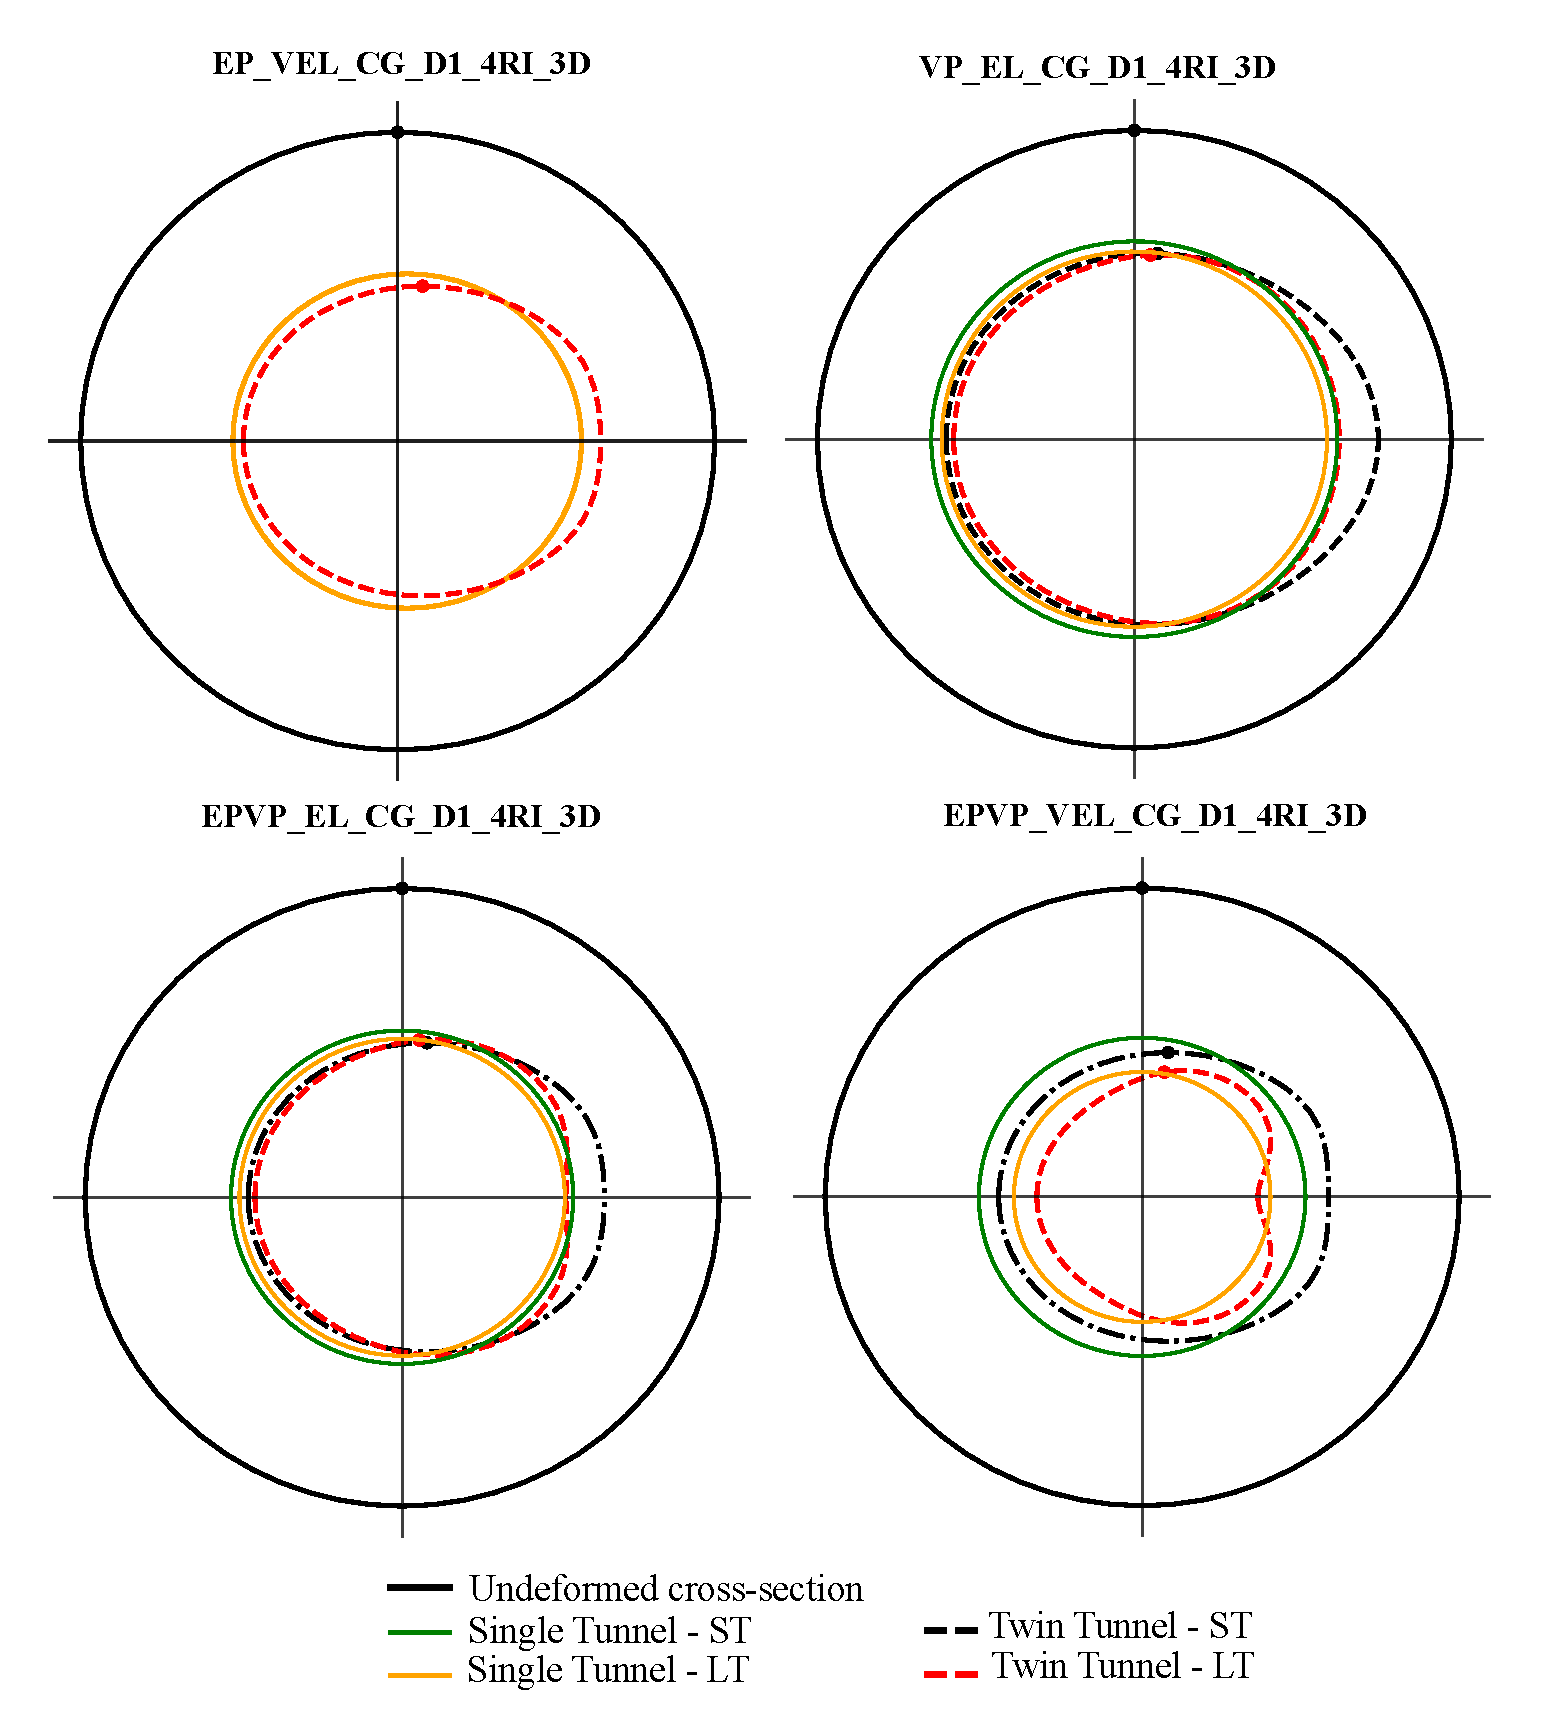
\includegraphics[scale=0.4]{ovalization.pdf}
	\caption{Ovalization effect for $d_1 = 4R_t$ with deformations magnified 50x.}
	\label{ovalization}
\end{figure}
\FloatBarrier
Figs.~\ref{UB-UAUB-D1_4RT} show ovalization effect $U_B/U_A = u_y(B)/u_x(A)$ between the vertical displacement $u_y$ at the roof B and the horizontal displacement $u_x$ at the side wall $A(x=R_t,y=0,z)$, for $d_1 = 4R_t$ without gallery. The effect is more pronounced in the short-term (solid lines).
\begin{figure}[h!]
	\centering
	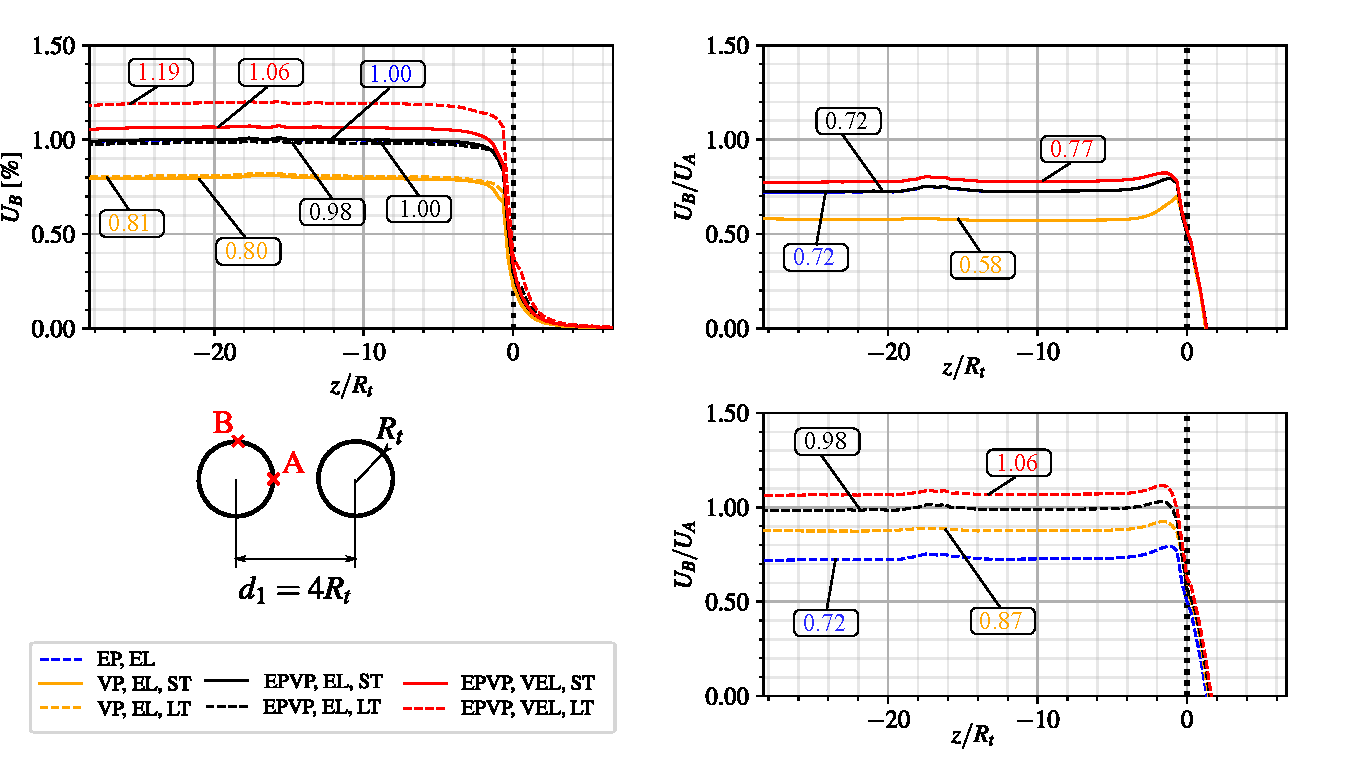
\includegraphics[scale=0.65]{Convergence Profiles - UB - UAUB - $d_1=4R_t - ST_Lt$.pdf}
	\caption{Convergence Profiles - ovalization effect for $d_1 = 4R_t$ without gallery.}
	\label{UB-UAUB-D1_4RT}
\end{figure}
\FloatBarrier

\subsection{Long-term analysis with viscous models}\label{}

Fig.~\ref{VP-EL-EPVP-VEL-WG-LT} shows the convergence profiles for $d_1 = 16R_t, 8R_t$ and $4R_t$ (yellow, green and red lines, respectively) with viscous constitutive models: viscoplastic rock mass with elastic lining (VP-EL - solid lines), elastoplastic-viscoplastic rock mass with elastic lining (EPVP-EL - dashed line) and viscoelastic lining (EPVP-VEL - dotted lines). As a reference, it also shows the results of a single tunnel (black lines). A slight increase in the peak value of convergence $U_{peak}$ can be seen for the EPVP-VEL model when comparing $d_1 = 16R_t$ (yellow dotted line) and $d_1 = 8R_t$ (green dotted line). In the case of $d_1 = 8R_t$, the proximity of the tunnel compensates the convergence difference due the gallery excavation eplapsed time between $d_1 = 8R_t$ and $16 R_t$. However, when $d_1 = 4R_t$ (red  dotted line) the effect of the gallery is more pronounced due to the interaction between the proximity of the twin tunnels and the viscous effect. 

Moreover, it is possible to observe higher convergence values in the excavated length that precedes the excavation of the gallery, specifically, in the EPVP-VEL model for $d_1 = 8R_t$ and $d_1 = 16R_t$ (green and yellow dotted lines). This effect is due to the viscoelastic behavior of the lining during the elapsed time to excavate the gallery. Unlike the highly rigid elastic lining, the viscoelastic lining allows the convergence to evolve during the excavation of the gallery. Consequently, the values of convergences before the gallery tend to be higher than after the gallery.

\begin{figure}[h!]
	\centering
	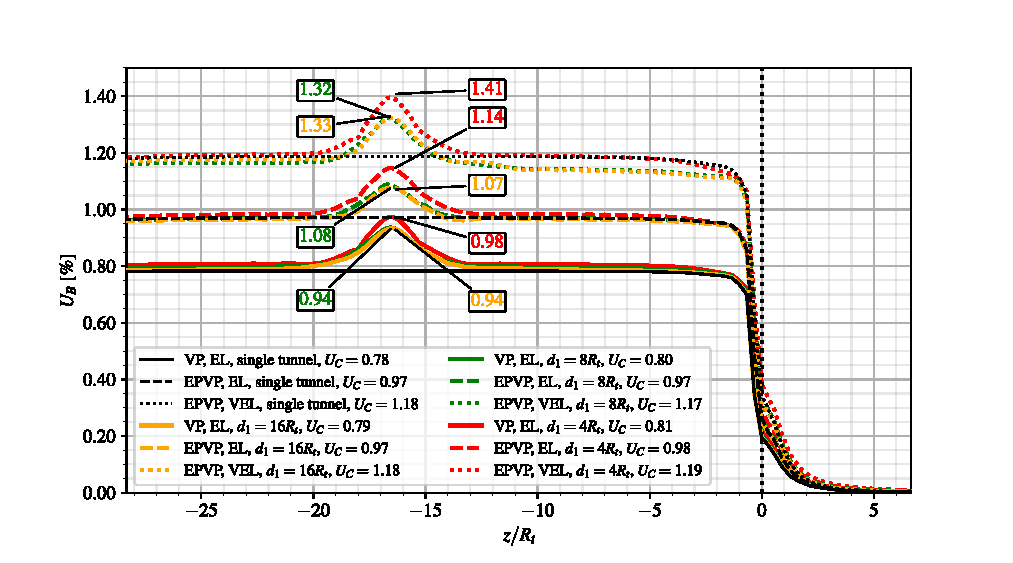
\includegraphics[scale=0.9]{Convergence Profiles - VP_EPVP_EL_VEL_WG_LT_anotate.pdf}
	\caption{Convergence Profiles - viscoplastic rock mass (VP) with elastic lining (EL) compared to elastoplastic-viscoplastic rock mass (EPVP) with elastic (EL) and viscoelastic lining (VEL) in long-term (LT).}
	\label{VP-EL-EPVP-VEL-WG-LT}
\end{figure}
\FloatBarrier

Fig.~\ref{EP-EL-EPVP-VEL-WG-ST-LT} shows the convergence profiles for $d_1 = 16R_t, 8R_t$ and $4R_t$ (yellow, green and red lines, respectively) with elastoplastic rock mass with elastic lining (EP-EL - solid lines), elastoplastic-viscoplastic rock mass with viscoelastic lining in short-term (EPVP-VEL-ST - dotted lines) and long-term (EPVP-VEL-LT - dashed lines). As a reference, it also shows the results of a single tunnel (black lines). 

\begin{figure}[h!]
	\centering
	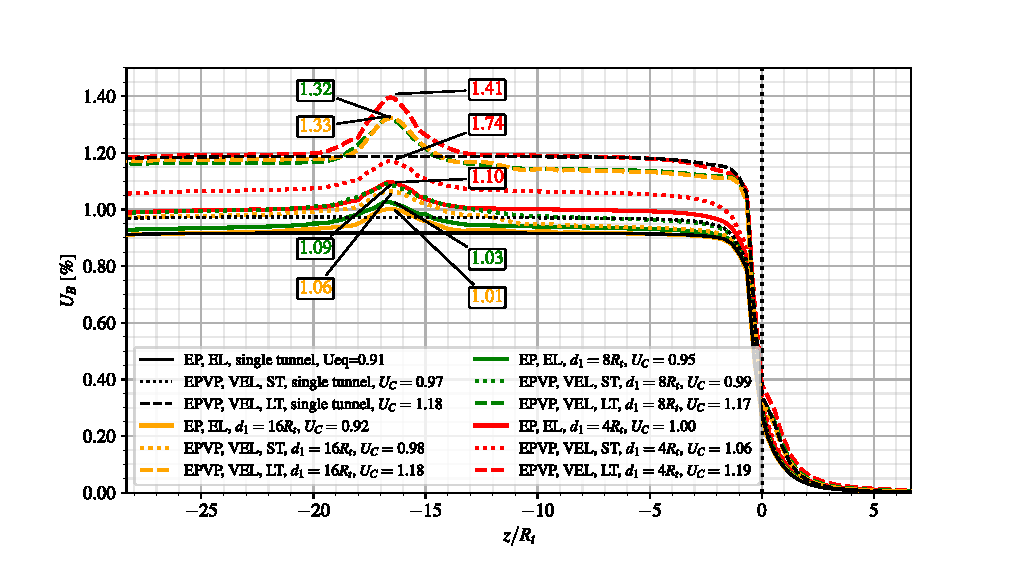
\includegraphics[scale=0.9]{Convergence Profiles - EP_EL_EPVP_VEL_WG_ST_LT_anotate.pdf}
	\caption{Convergence Profiles - elastoplastic rock mass (EP) with elastic lining (EL) compared to elastoplastic-viscoplastic rock mass (EPVP) with viscoelastic lining (VEL) in short-term (ST) and long-term (LT).}
	\label{EP-EL-EPVP-VEL-WG-ST-LT}
\end{figure}
\FloatBarrier

The results show the crucial effect of the viscoelastic lining to the convergence profile of the tunnels. In the short-term (ST), the elastoplastic-viscoplastic rock mass with viscoelastic lining (EPVP-VEL - dotted lines) shows higher convergences compared to the elastoplastic with elastic lining (EP-EL - solid lines). Because the early age of the viscoelastic lining (VEL) has a lower modulus of elasticity, resulting in lower stiffness. Therefore, compared to the elastic lining (EL), the lower initial value of the modulus of elasticity contributes more to the development of convergence. In the long-term (LT), even though the viscoelastic lining (VEL) (dashed lines) has a higher stiffness due to the aging of lining, the viscous effects over time result in a significantly more discrepant convergence profile compared to the elastoplastic with elastic lining (EP-EL - solid lines). There is a noticeable increase in the magnitude of $U_{peak}$ between the short-term (dotted lines) and the long-term (dashed lines) at the gallery position, highlighting the influence of the viscoelastic lining.

\subsection{Effect of lining stiffness on convergence evolution}\label{}

To study the effect of the lining stiffness, Fig.~\ref{EP_d1_16Ri} and \ref{EP_d1_4Ri} show the elastoplastic rock mass (EP) under various conditions: without lining (NL - dashed lines), with a moderately stiff elastic lining ($K_c = 969$ MPa - dotted lines), and with a higher stiff elastic lining ($K_c = 3403$ MPa - solid lines) with gallery (WG - blue lines) and without gallery (NG - yellow lines) for $d_1 = 16R_t$ and $4R_t$, respectively. As a reference, it also shows the results of a single tunnel (black lines). The stiffness values, $K_c = 969$ MPa and $K_c = 3403$ MPa, are obtained from following expression in [\citenum{Panet1995}] for single tunnels, considering Young's modulus at 28 days $E_c = 30303$ MPa, Poisson's ratio $\nu_c = 0.2$ and lining thickness of $0.03R_t$ and $0.1R_t$, respectively.
\begin{equation} \label{eq:8}
	K_c = \frac{E_c}{1+\nu_c}\frac{R_t^2-(R_t-e_t)^2}{(1-2\nu_c)R_t+(R_t-e_t)^2}
\end{equation}
\begin{figure}[h!]
	\centering
	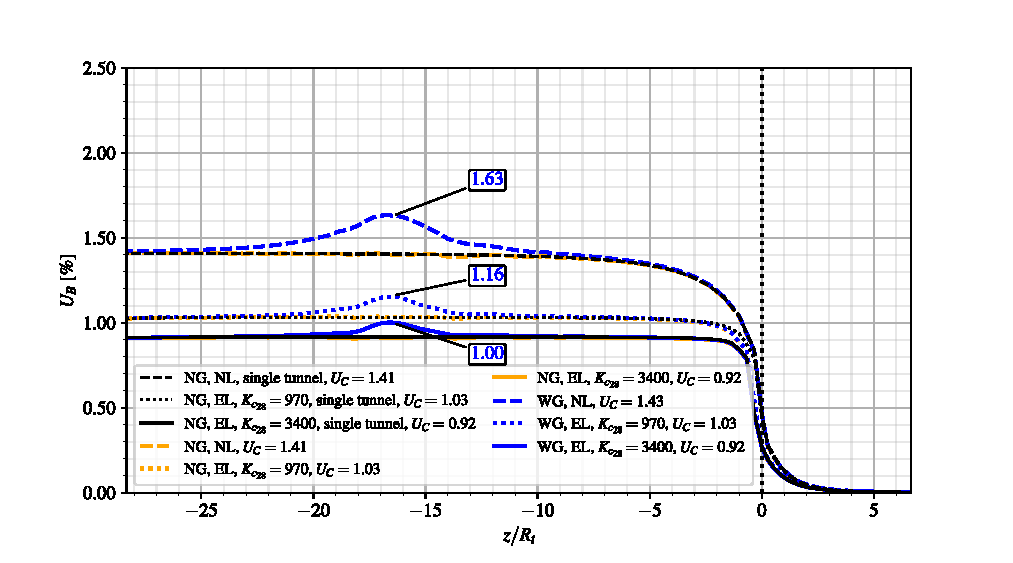
\includegraphics[scale=0.9]{Convergence Profiles - EP_d1_16Ri_anotate.pdf}
	\caption{Convergence Profiles - elastoplastic rock mass (EP) without lining (NL) with a higher stiff elastic lining ($K_c = 3403$ MPa) and a moderately stiff elastic lining ($K_c = 969$ MPa), without (NG) and with gallery (WG) for $d_1 = 16R_t$.}
	\label{EP_d1_16Ri}
\end{figure}
\FloatBarrier
\begin{figure}[h!]
	\centering
	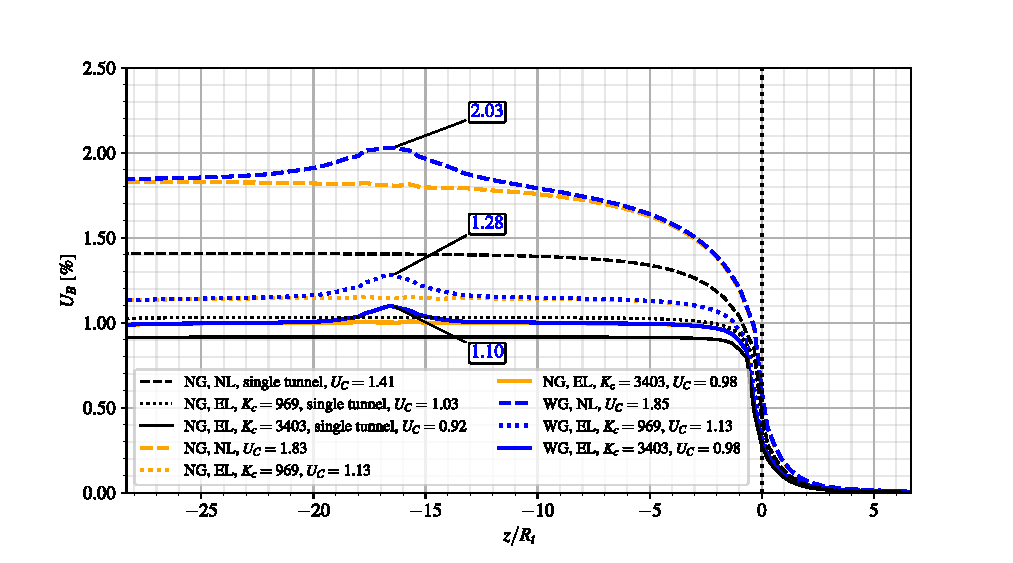
\includegraphics[scale=0.9]{Convergence Profiles - EP_d1_4Ri_anotate.pdf}
	\caption{Convergence Profiles - elastoplastic rock mass (EP) without lining (NL) with a higher stiff elastic lining ($K_c = 3403$ MPa) and a moderately stiff elastic lining ($K_c = 969$ MPa), without (NG) and with gallery (WG) for $d_1 = 4R_t$.}
	\label{EP_d1_4Ri}
\end{figure}
\FloatBarrier

For the single tunnel, the higher stiffness lining (black solid line) reduced convergence by approximately 35\% compared to the unlined scenario (black dashed line). Conversely, the moderately stiff lining (black dotted line) increases convergence by 12\% compared to the rigid lining. 

When $d_1 = 16R_t$ (blue and yellow lines), the results of $U_{C}$ are similar to the isolated tunnel (black line). However, with a distance reduced to $d_1 = 4R_t$, the interaction between the tunnels becomes significant. A smaller $d_1$, the high stiffness lining (yellow and blue solid lines) can restrict convergence by up to 46\% of the unlined convergence (yellow and blue dashed lines). A moderate stiffness lining (dotted lines) leads to an increase of up to 16\% in convergence compared to the higher stiffness lining (solid lines).

When comparing results between twin lined tunnels with $d_1 = 16R_t$ and $4R_t$, differences of 6\% with higher stiffness lining (yellow and blue solid lines), 10\% with moderate stiffness lining (yellow and blue dotted lines), and 30\% without lining (yellow and blue dashed lines) are observed. These results show the direct impact of lining stiffness and the distance between twin tunnels on $U_{C}$ convergence.

When analyzing the convergence $U_{peak}$ at the point where the gallery meets the longitudinal tunnel, there is an increase of 16\% when using a moderate stiffness lining (dotted blue line) compared to a higher stiffness lining (blue solid line). However, when analyzing the difference between the $U_{C}$ and $U_{peak}$, there is a difference of up to 12\% for the higher stiffness lining (blue solid line to $4R_t$ and $16R_t$) and up to 13\% for the moderate stiffness lining (blue dotted line to $4R_t$ and $16R_t$) for $d_1=4R_t$. In all cases, the increase in stiffness reduces the extent of the disturbed region caused by the gallery in the longitudinal tunnel convergence profile. The range decreases from 22.5$R_g$ (without lining) to 10.5$R_g$ and 7.5$R_g$ (with lining). Additionally, the proximity of the longitudinal tunnels has a minimal impact on the length of this gallery influence zone.

In line with the previous analysis of lining stiffness, Fig.~\ref{EPVP_VEL_d1_16Ri} and Fig.~\ref{EPVP_VEL_d1_4Ri} present the results for elastoplastic-viscoplastic rock mass (EPVP), considering a viscoelastic lining (VEL) with (WG - blue lines) and without gallery (NG - yellow lines) for $d_1 = 16R_t$ and $4R_t$, respectively. For reference, results for a single tunnel are also included (black lines). This analysis aims to assess the influence of the lining stiffness, particularly when twin tunnels are in close proximity. 

The results indicate that, once again, the convergence profile under these conditions, with a distance of $16R_t$ between the tunnels, closely resembles that of an isolated tunnel. Differences are on the order of 1.8\% for a moderately stiff lining and 0.8\% for a higher stiff lining.
\begin{figure}[h!]
	\centering
	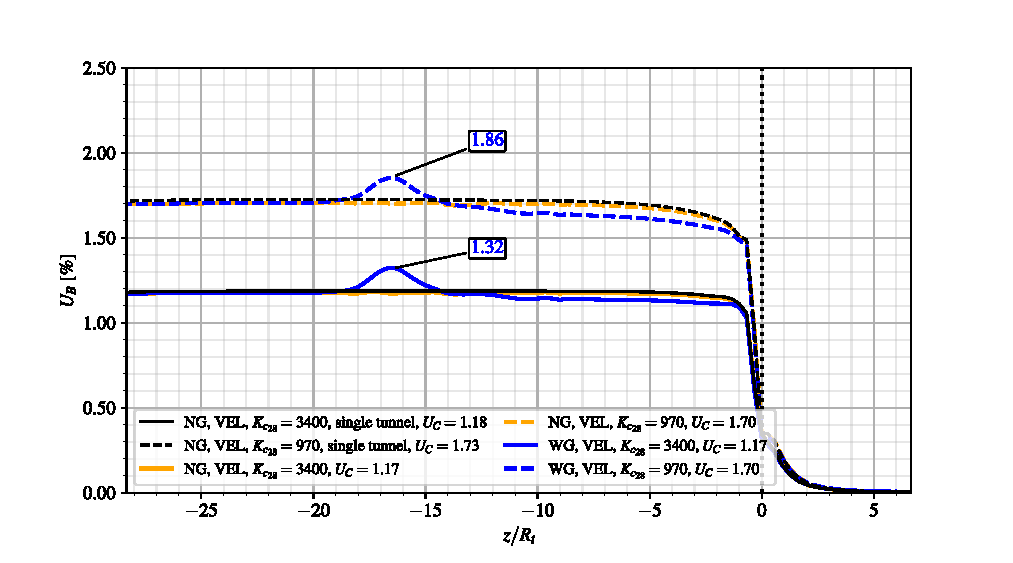
\includegraphics[scale=0.9]{Convergence Profiles - EPVP_VEL_d1_16Ri_anotate.pdf}
	\caption{Convergence Profiles - elastoplastic-viscoplastic rock mass (EPVP) with a higher stiff viscoelastic lining ($K_c = 3403$ MPa) and a moderately stiff viscoelastic lining ($K_c = 969$ MPa), without (NG) and with gallery (WG) for $d_1 = 16R_t$.}
	\label{EPVP_VEL_d1_16Ri}
\end{figure}
\FloatBarrier
\begin{figure}[h!]
	\centering
	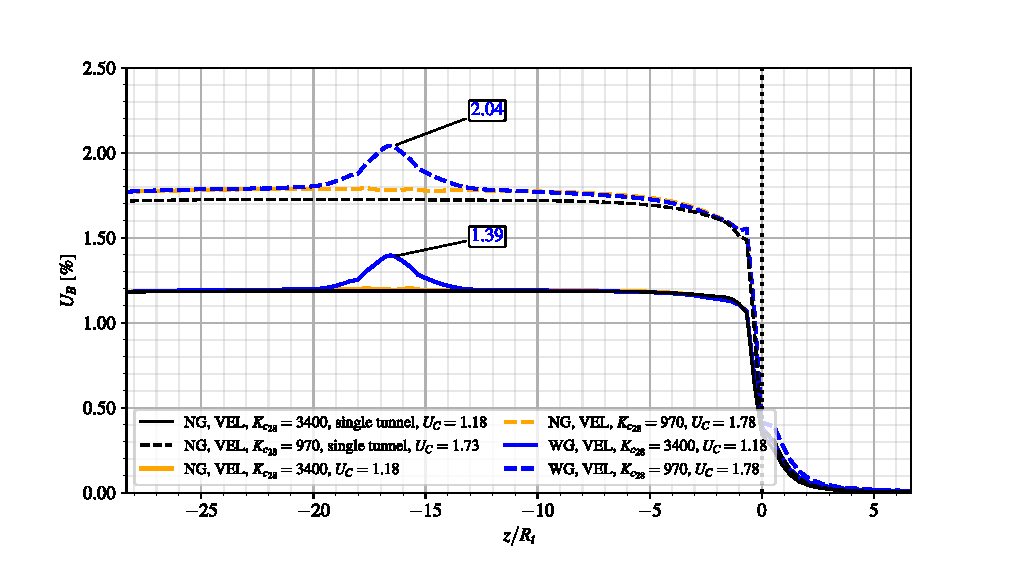
\includegraphics[scale=0.9]{Convergence Profiles - EPVP_VEL_d1_4Ri_anotate.pdf}
	\caption{Convergence Profiles - elastoplastic-viscoplastic rock mass (EPVP) with a higher stiff viscoelastic lining ($K_c = 3403$ MPa) and a moderately stiff viscoelastic lining ($K_c = 969$ MPa), without (NG) and with gallery (WG) for $d_1 = 4R_t$.}
	\label{EPVP_VEL_d1_4Ri}
\end{figure}
\FloatBarrier

In the case of $d_1=4R_t$, when the higher stiffness lining is applied (blue and yellow solid lines), there is practically no difference compared to the single tunnel (black solid line). This occurs because the higher stiffness of the lining blocks convergence in the interaction between the tunnels. However, when using a moderately stiff lining (blue and yellow dashed lines), there is a difference of approximately 3\% in the convergence $U_{C}$ compared to the single tunnel (black dashed line).

When comparing the results for $d_1 = 16R_t$ and $4R_t$, considering each lining separately, there is a difference of 0.8\% when there is a higher stiffness lining (solid yellow and blue lines to $16R_t$ and $4R_t$) and 4.8\% for a moderate stiffness lining (dashed yellow and blue lines to $16R_t$ and $4R_t$). Thus, once again, the importance of the stiffness of the lining when associated with the distance between the twin tunnels.

When analyzing the convergence $U_{peak}$ at the point where the gallery meets the longitudinal tunnel, there is an increase of 47\% for $d_1=4R_t$ when using an moderate stiffness lining (dashed blue line) compared to a high stiffness lining (solid blue line). However, when analyzing the difference between the $U_{C}$ and $U_{peak}$, there is a difference of up to 18\% for the high stiffness lining (solid blue line) and up to 15\% for the moderate stiffness lining (dashed blue line) for $d_1=4R_t$.

The following results (Figs.~\ref{EPVP_EL_VEL_d1_16Ri} and ~\ref{EPVP_EL_VEL_d1_4Ri}) compare the elastic (EL - dashed and solid lines) and viscoelastic (VEL - dotted line) lining, considering the elastoplastic-viscoplastic model (EPVP) for the rock mass. 
\begin{figure}[h!]
	\centering
	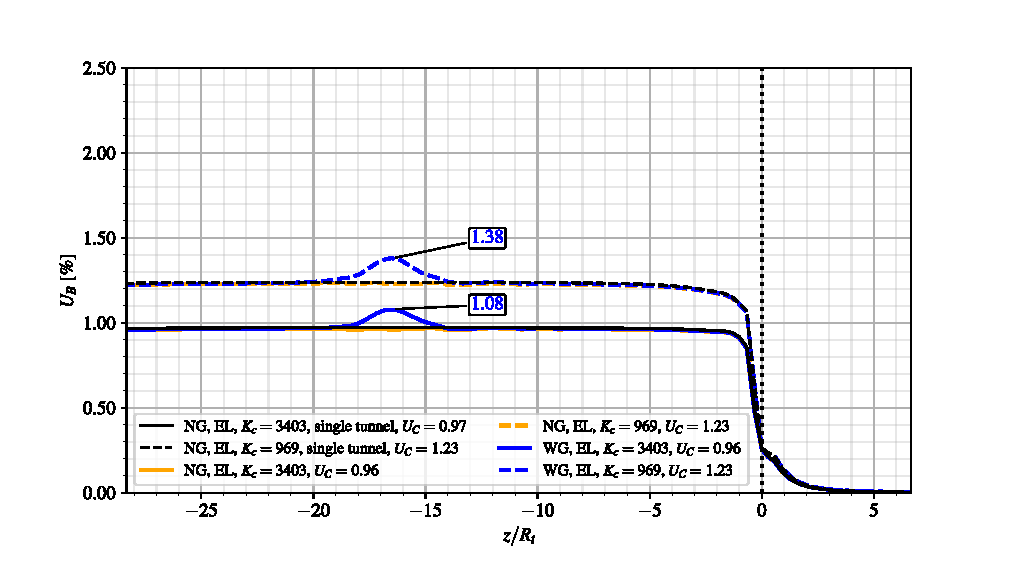
\includegraphics[scale=0.9]{Convergence Profiles - EPVP_EL_VEL_d1_16Ri_anotate.pdf}
	\caption{Convergence Profiles - elastoplastic-viscoplastic rock mass (EPVP) without lining (NL) with a higher stiff ($K_c = 3403$ MPa) and a moderately stiff ($K_c = 969$ MPa) elastic (EL) and viscoelastic (VEL) lining, without (NG) and with gallery (WG) for $d_1 = 16R_t$.}
	\label{EPVP_EL_VEL_d1_16Ri}
\end{figure}
\FloatBarrier
\begin{figure}[h!]
	\centering
	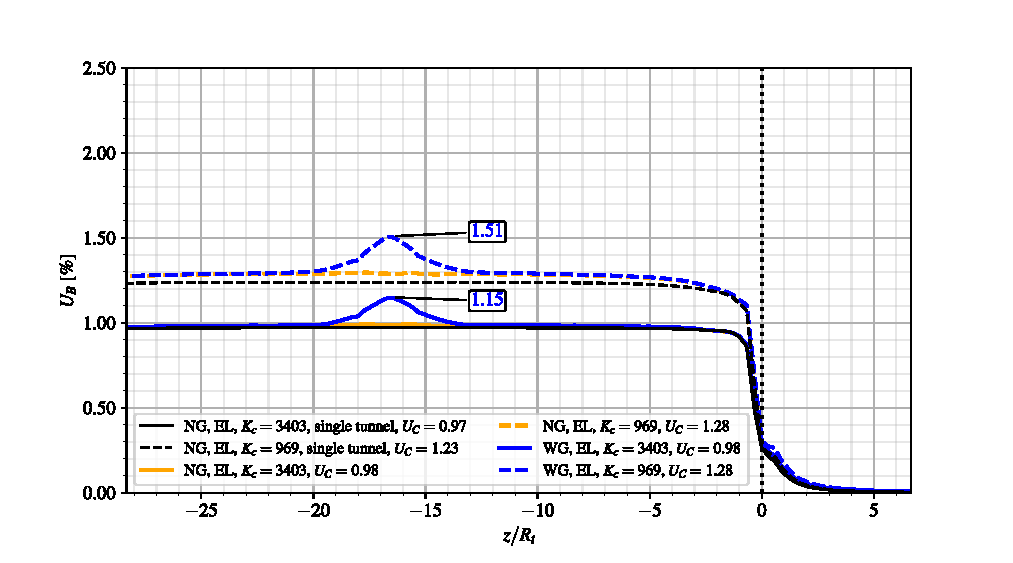
\includegraphics[scale=0.9]{Convergence Profiles - EPVP_EL_VEL_d1_4Ri_anotate.pdf}
	\caption{Convergence Profiles - elastoplastic-viscoplastic rock mass (EPVP) without lining (NL) with a higher stiff ($K_c = 3403$ MPa) and a moderately stiff ($K_c = 969$ MPa) elastic (EL) and viscoelastic (VEL) lining, without (NG) and with gallery (WG) for $d_1 = 4R_t$.}
	\label{EPVP_EL_VEL_d1_4Ri}
\end{figure}
\FloatBarrier
For $d_1 = 16R_t$, the most significant difference in $U_{C}$ compared to the isolated tunnel (black dotted line) occurs with the moderately stiff viscoelastic lining (blue dotted line), showing an increase of approximately 1.8\%. In contrast, for $d_1 = 4R_t$, the differences increase to 4\% for the elastic lining (dashed lines) and 3\% for the moderately stiff viscoelastic lining (dotted lines). Using the higher stiffness elastic lining as a reference (solid lines), for $d_1 = 16R_t$, the differences rise to 27\% for the elastic (dashed lines) and 78\% for viscoelastic (dotted lines) lining with moderate stifness. For $d_1 = 4R_t$, these differences further increase to 31\% and 81\%, respectively.

When analyzing the convergence at the peak $U_{peak}$, which corresponds to the point where the gallery meets the longitudinal tunnel, and using the value of the higher stiffness elastic lining (solid lines) as the reference, an increase of up to 31\% and 77\% is observed for $d_1=4R_t$ when using the elastic (dashed lines) and viscoelastic (dotted lines) linings of moderate stiffness, respectively. However, when analyzing the difference between the $U_{C}$ and $U_{peak}$, there is a difference of up to 18\% for the moderate stiffness elastic lining (blue dashed line) and up to 15\% for the moderate stiffness viscoelastic lining (blue dotted line) for $d_1=4R_t$.

Finally, Fig.~\ref{EP_EPVP_NG_LT_single tunnel} shows a comparison between the elastic and viscoelastic lining, considering higher (solid lines) and moderate stiffness (dotted lines), and between the elastoplastic (black lines) and elastoplastic-viscoplastic (red and blue) rock mass. Results without the lining (NL - dashed lines) are also included.
\begin{figure}[h!]
	\centering
	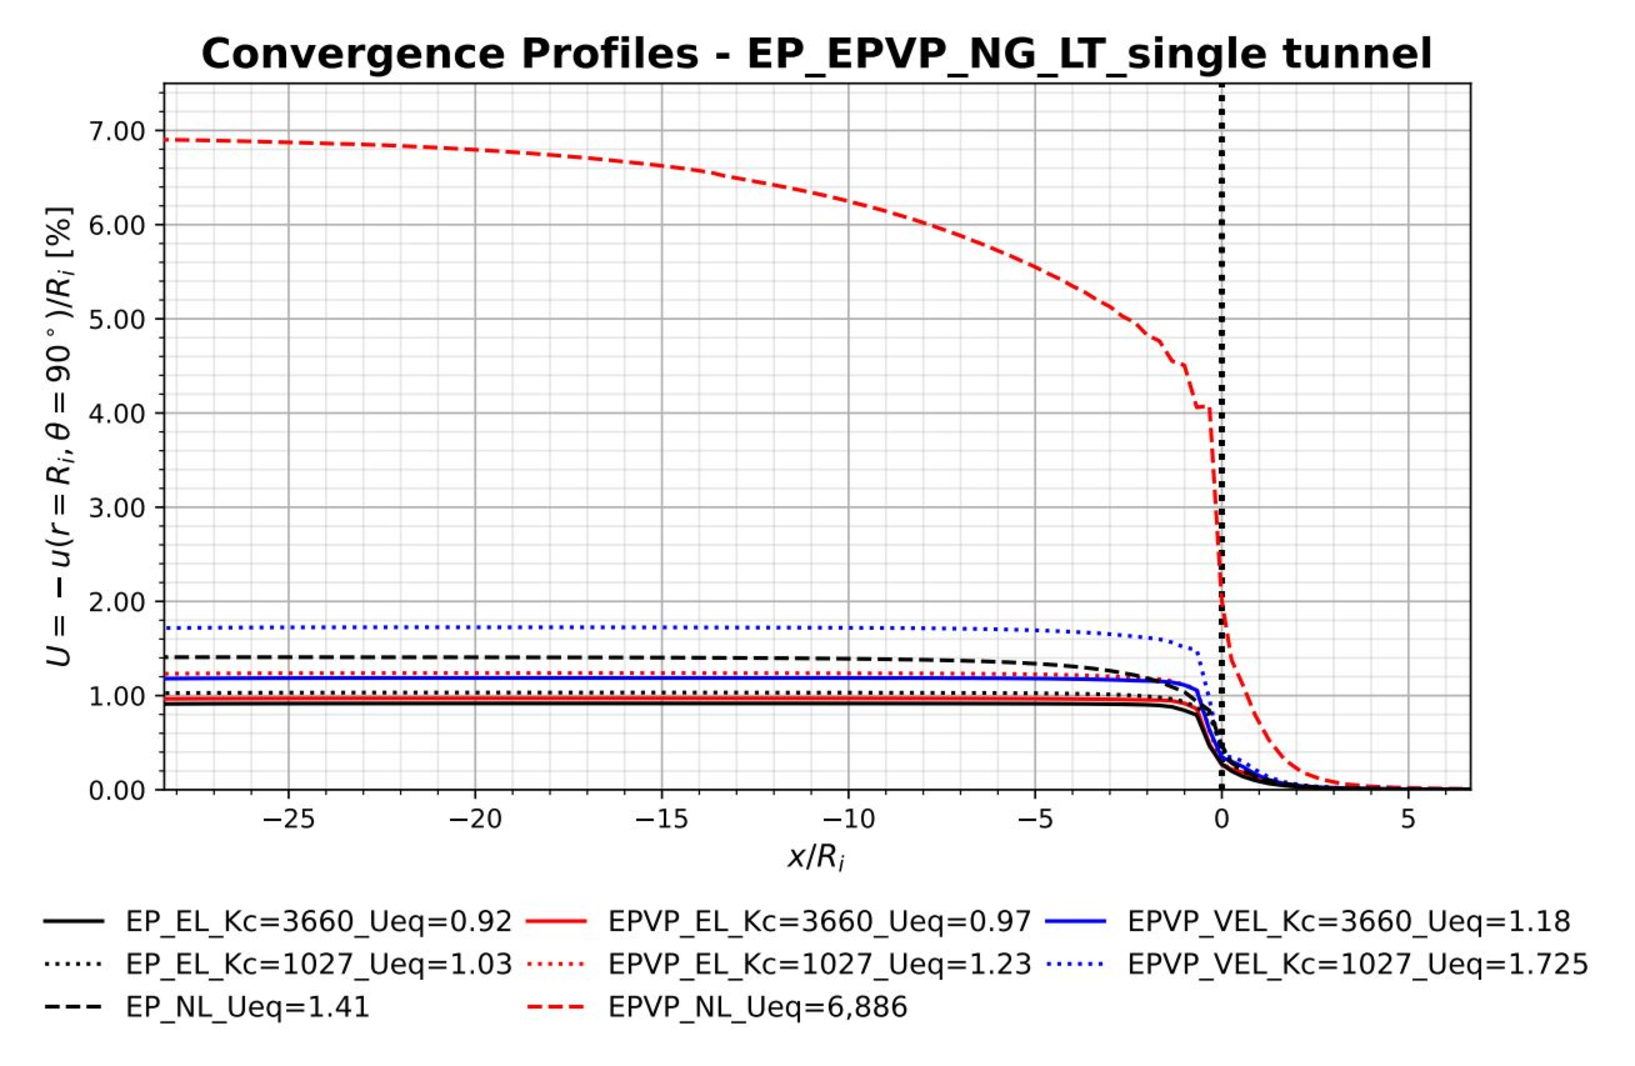
\includegraphics[scale=0.7]{Convergence Profiles - EP_EPVP_NG_LT_single tunnel.pdf}
	\caption{Convergence Profiles - single tunnel with elastoplastic (EP) and elastoplastic-viscoplastic rock mass (EPVP), without lining (NL) with a higher stiff ($K_c = 3403$ MPa) and a moderately stiff ($K_c = 969$ MPa) elastic (EL) and viscoelastic (VEL) lining.}
	\label{EP_EPVP_NG_LT_single tunnel}
\end{figure}
\FloatBarrier
Taking as a reference the elastoplastic model with the higher stiffness lining (solid black line) we observed a difference of 12\% and 53.5\%, respectively, in the cases of the elastoplastic rock mass with an elastic lining of moderate stiffness (dotted black) and without a lining (dashed black line), respectively. We also identified a difference of 5.5\%, 33.5\%, and 748\% when using the elastoplastic-viscoplastic rock mass with an elastic lining of higher stiffness (solid red line), moderate stiffness (dotted red line), and no lining (dashed red line), respectively. In addition, we found a difference of 28\% and 87.5\% when comparing with the elastoplastic-viscoplastic rock mass with the higher stiffness (solid blue line) and moderate stiffness viscoelastic lining (dotted blue line), respectively.

\section{Conclusions}\label{}

In general, the field of deformations and stresses around a deep tunnel depends on several interrelated factors, including the tunnel depth, anisotropy of in situ stresses, tunnel wall geometry, tunneling conditions, and the mechanical behavior and coupling of the rock mass and the lining. In twin tunnels, there is also the interaction due to the proximity between the tunnels and, if present, transverse galleries, which cause localized stress distribution and overloading the main tunnels. Furthermore, unlike single tunnels, the gallery's influence can only be studied with three-dimensional models.

One of the contributions of this study at the structural level is the development of a model capable of performing three-dimensional finite element simulations for a domain of deep circular twin tunnels with a transverse gallery. The construction process, including excavation and lining installation, was simulated using an activation/deactivation technique. At the material level, four constitutive models for the rock mass were implemented and investigated: elastic (E), elastoplastic (EP), viscoplastic (VP), and elastoplastic-viscoplastic (EPVP) model. For the lining, three configurations were considered: no lining (NL), elastic (EL), and viscoelastic (VEL). In the numerical application of this study, the influence of different constitutive models was explored, as well as the effect of the spacing between axes of the longitudinal tunnels ($d_1 = 16R_t$, $8R_t$ and $4R_t$ where $R_t$ is the tunnel radius) and the impact of lining stiffness on deformation control. For time-dependent models (which account for rock mass creep and lining creep and shrinkage), results were obtained and analyzed at the end of tunnel construction (short-term - ST) and after viscous effects had reached equilibrium (long-term - LT).

However, before this application, preliminary numerical simulations of the 3D computational model were carried out, and comparisons were made with analytical solutions for unlined twin tunnels under plane strain conditions, considering both elastic and elastoplastic rock mass. These simulations demonstrated the model's capacity to accurately capture the main effects occurring in such structures, including the ovalization effect, stress distribution, and the extent of the plastic zone, for various tunnel spacing, initial in situ stresses, and different values of cohesion and friction angle.

Regarding the application of this study, the main objective was to demonstrate the capability of the proposed formulation to address the three-dimensional problem of twin tunnels connected to galleries, involving nonlinear and time-dependent behaviors. However, a comprehensive parametric analysis that integrates the effects of geometric, constitutive, and loading parameters is beyond the scope of this specific numerical application. Constitutive parameters were selected for deep clay rockmass (at a depth of 450 m) from the eastern Paris basin, based on laboratory tests conducted under undrained conditions, which exhibited both instantaneous and delayed behavior and could be simulated by the implemented constitutive models. For the lining of both the twin tunnels and the gallery, a constitutive model values was used that takes into account the creep and shrinkage of concrete, through a viscoelastic aging model.

Considering the constitutive parameters and tunneling conditions adopted, some conclusions from this study can be highlighted. First, when comparing the convergence profiles, the difference between short-term and long-term responses is more pronounced when the lining is viscoelastic. This demonstrates the importance of adopting a model that accounts for concrete creep and shrinkage. The relatively high stiffness of an elastic lining significantly reduces the viscous deformations. In the short-term, the early age of the lining results in a lower relaxation modulus compared to the constant 28-day modulus used for the elastic lining. In the long-term, although the viscoelastic lining shows an increase in the relaxation modulus due to the aging phenomenon, the creep of both the rock and the lining components results in significantly greater convergences compared to models that do not consider time-delayed effects.

Additionally, the results indicate that the ovalization effect on the tunnel wall, caused by the proximity between the tunnels, is more pronounced in the short term. Over time, the viscosity of the rock mass tends to reduce this ovalization effect. The impact on tunnel convergence, due to the proximity of the tunnels $d_1$ and the time required for the complete excavation of the gallery, which also depends on this proximity, was most significant for a distance of $d_1 = 4R_t$. This distance resulted in the highest peak convergence value at the roof of the longitudinal tunnel, located at the intersection of the twin tunnels' axes and the gallery, represented by $U_{peak}$. Furthermore, a significant increase in the magnitude of $U_{peak}$ between the short-term and long-term responses was observed, due to the influence of the time-dependent behavior of the rock and the lining.

To assess the effect of the lining stiffness on deformation control, complementary analyses were carried out by reducing the lining thickness from $0.1R_t$ (higher stiffness) to $0.03R_t$ (moderate stiffness). Considering the elastoplastic behavior of the rock mass, the stiffer lining resulted in a 35\% reduction in convergence compared to the unlined structure, while the moderate stiffness lining reduced convergence by only 12\%. Regarding the influence zone of the gallery on the longitudinal tunnel convergence profile, it was observed that increasing the stiffness reduced the extent of this zone in all studied configurations. However, the spacing $d_1$ between the tunnels had little impact. In the configuration with the largest spacing $d_1 = 16R_t$, where less interaction between the twin tunnels is expected, the relative variation between the peak convergence $U_{peak}$ and the convergence outside the gallery’s influence zone $U_c$ was approximately 14\% for the unlined structure, 12.5\% for the moderate stiffness lining, and 8.7\% for the stiffer lining. These values were reduced to 9.7\%, 13\%, and 12\%, respectively, for the spacing of $d_1 = 4R_t$, where the effects of lining stiffness and tunnel proximity occur simultaneously.

When the rock mass is elastoplastic-viscoplastic, long-term results suggest that the extent of the influence zone is also not affected by the distance $d_1$. However, the difference between the peak convergence $U_{peak}$ and the convergence outside the gallery's influence zone $U_c$ is significantly influenced by $d_1$ and the stiffness of the lining. For an elastic lining, this difference is 12\% for $d_1 = 16R_t$ and 18\% for $d_1 = 4R_t$. This confirms that the effect of tunnel proximity on peak convergence is predominant. However, when the lining is viscoelastic, the stiffness of the lining significantly influences this difference. For $d_1 = 16R_t$, the values are 9.5\% for the moderate stiffness lining and 13\% for the stiffer lining. For $d_1 = 4R_t$, these values are 14.5\% and 18\%, respectively, indicating the complex interaction between tunnel proximity, the gallery, and nonlinear constitutive models.

%The fundamental role of the stiffness of the concrete lining in the convergence profile of twin tunnels is understood from the analyses. Depending on the value of this stiffness, it is possible to condition the restriction of viscous effects that tend to manifest over time after the completion of the excavation process.

%Additionally, the effect of the interaction between longitudinal tunnels is notable when considering proximity, with major influence from a distance of 4 radii. However, in many cases, this effect may be subtle or almost imperceptible due to the presence of a higher rigid lining.

%In models considering the viscosity of the rock mass, the time factor plays a significant role in convergence. In this scenario, when excavating the gallery with $d_1 = 16R_t$, the portion of the tunnel already excavated remains subject to viscous effects for a more extended period compared to other distances. In any case, when $d_1 = 4R_t$, the proximity interaction between twin tunnels, along with viscous effects over time, results in a higher value compared to cases where $d_1 = 16R_t$ and $8R_t$.

%Another important observation related to EPVP-EL and EPVP-VEL models concerns the possible ovalization of the section over time, concerning the analyzed reference point on the section perimeter (in the crown). Instead of following the logic of following the closing direction of the section, it may undergo some negative displacement in the long-term. The result, for the same observation point, is a convergence value that in the short-term may indicate section closure but in the long-term may indicate the opposite.

%Another crucial observation regarding EPVP-EL and EPVP-VEL models pertains to the potential ovalization of the section over time, particularly concerning the analyzed reference point on the section perimeter (in the crown). Instead of conforming to the expected logic of closing in the section's direction, it might experience negative displacement in the long-term. Consequently, for the same observation point, the convergence value may initially suggest section closure in the short-term but indicate the opposite in the long-term.

%Concerning the EPVP-VEL model, specifically with distances of 16 and 8 radii between twin tunnels, we observe that Ueq in the section ahead of the gallery region is slightly smaller than Ueq in the section preceding the gallery. This variation in the convergence profile results from the shorter exposure time to viscous effects in the portion excavated later than the transverse gallery. Therefore, during the gallery excavation process, the portion of the longitudinal tunnel already excavated experiences viscous effects until completing the gallery excavation. 

%However, concerning the existence of a transverse gallery and adopting the constitutive parameters while considering the presence of lining, its influence is highly localized, spanning approximately four radii on each side from its axis. Consequently, there is no significant impact on the remaining convergence profile of the tunnels, except for the model with viscoelastic lining, where lower convergences occur after the gallery. 

%% To print the credit authorship contribution details
%\printcredits
%
%%% Loading bibliography style file
%%\bibliographystyle{model1-num-names}
\bibliographystyle{model3-num-names}
%\bibliographystyle{elsarticle-num-names}
%
%% Loading bibliography database
\bibliography{cas-refs}
%
%% Biography
%\bio{}
%% Here goes the biography details.
%\endbio
%
%\bio{pic1}
%% Here goes the biography details.
%\endbio

\end{document}

